\documentclass[10pt,handout]{beamer}

\usepackage[spanish]{babel}
\usepackage[utf8]{inputenc} 
\usepackage[T1]{fontenc}
\usepackage{lmodern}

%\usepackage{beamerthemebars}
\usepackage{pythontex}
\usepackage{graphics}
\usepackage{hyperref}
\usepackage{multimedia}
\usepackage{tikz}
\usetikzlibrary{fpu}
%\usepackage[french]{babel}

\usepackage{latexsym} % Símbolos                        ı
\usepackage{amsmath}
\usepackage{amssymb}
\usepackage{listings}
\usepackage{pgfplots}

\pgfplotsset{every axis/.append style={
    axis x line=middle,    % put the x axis in the middle
    axis y line=middle,    % put the y axis in the middle
    axis line style={<->}, % arrows on the axis
    xlabel={$x$},          % default put x on x-axis
    ylabel={$y$},          % default put y on y-axis
    },
    cmhplot/.style={color=red,mark=none,line width=1pt,<->},
    cmhplot1/.style={color=blue,mark=none,line width=1pt,<->},
    soldot/.style={color=red,only marks,mark=*},
    holdot/.style={color=red,fill=white,only marks,mark=*},
}

\tikzset{>=stealth}


\theoremstyle{plain} % default
  \newtheorem{thm}{Teorema}
\theoremstyle{plain} % default
  \newtheorem{lem}{Lema}
\theoremstyle{plain} % default
  \newtheorem{prop}{Proposici\'on}
\theoremstyle{plain} % default
  \newtheorem{cory}{Corolario}
\theoremstyle{definition}
  \newtheorem{defn}{Definici\'on}
\theoremstyle{example}
  \newtheorem{exmp}{Ejemplo}
\theoremstyle{example}
  \newtheorem{problema}{Problema}
\theoremstyle{remark}
  \newtheorem{respuesta}{Respuesta}
\theoremstyle{remark}
  \newtheorem{rem}{Nota}
%%%%%%%%%%%%%%%%%%%%%%%%%%%%
\spanishdecimal{.}
%\useoutertheme{infolines}
%\usetheme[compress]{Berlin}
\usetheme{default}
\useinnertheme{rectangles}
\useoutertheme{shadow}
\setbeamercovered{transparent}


\title{El Método de los Elementos Finitos}
\author{Antonio Falcó}
\date{Métodos Numéricos EDO-EDP}

\begin{document}

\begin{frame}
\maketitle
\end{frame}

\begin{frame}
  \tableofcontents
\end{frame}

\section{Introducción}

\subsection{Un problema modelo: La cuerda elástica}

\begin{frame}
\begin{itemize}
\item Estudiemos la deformación $u$ de una cuerda elástica sujeta por los extremos situados
en los puntos $x=0$ y $x=L$
\begin{center}
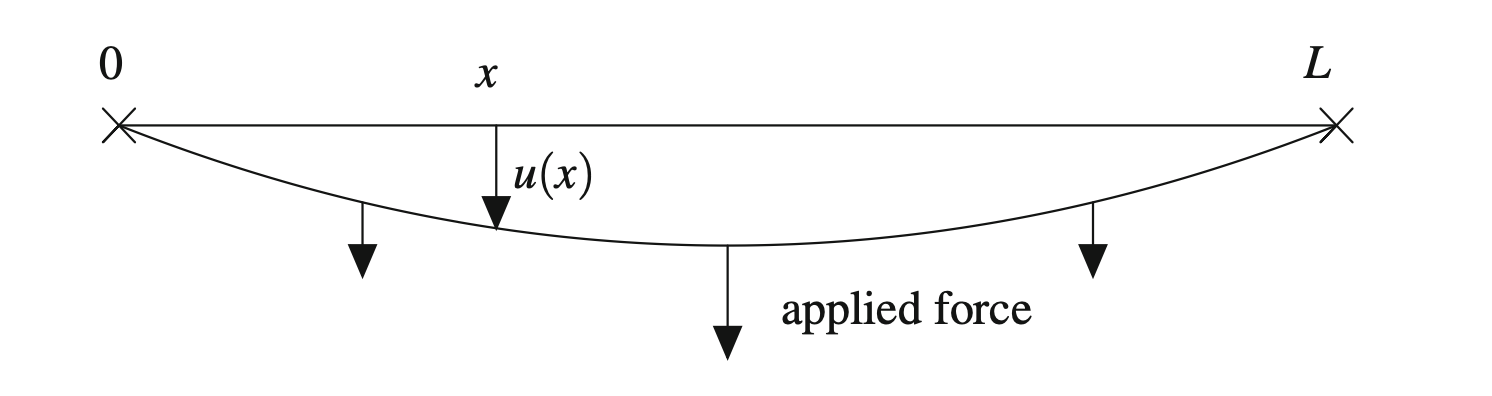
\includegraphics[scale=0.3]{./figure1.png}
\end{center}
\item La cuerda se deforma por efecto de las cargas. Estudiaremos el problema estático, en el que consideraremos 
que la cuerda se encuentra en equilibrio estático. Denotaremos por $u(x)$ la deformación vertical de 
la cuerda en la posición $0 \le x \le 1$ (esta deformación la supondremos, por hipótesis, estacionaria es decir independiente del tiempo).
\end{itemize}
\end{frame}

\begin{frame}
\begin{itemize}
\item El módulo de la tensión en cada punto $(x,0),$ que denotaremos simplemente por $x,$ de la cuerda es igual a  $T(x) = \|\mathbf{T}(x)\|.$
\item Si una fuerza vertical actua sobre la cuerda
$$\mathbf{F}(x) = \left( \begin{array}{c} 0 \\  \int_0^x f(s)ds  \end{array}\right),$$
donde $f:[0,L] \longrightarrow \mathbb{R}$ viene dada por
$f(x) = \rho(x)g$ donde $\rho(x)$ es la densidad de masa en $x.$
\item Si asumimos que la cuerda se encuentra en equilibrio se cumplirá que $\mathbf{T}(y)+\mathbf{F}(y)=\mathbf{T}(x)+\mathbf{F}(x),$ es decir:
$$
\mathbf{T}(y) - \mathbf{T}(x) + (\mathbf{F}(y) - \mathbf{F}(x)) = \mathbf{0} \text{ para todo } 0 \le x < y \le L
$$
\end{itemize}
\end{frame}

\begin{frame}
\begin{itemize}
\item Describiremos la cuerda deformada como una curva parametrizada por la posición $x:$
$$
\boldsymbol{\gamma}(x) = \left(
\begin{array}{c}
x \\ 
u(x)
\end{array}
\right)
$$
entonces
$$
\boldsymbol{\gamma}^{\prime}(x) = \left(
\begin{array}{c}
1 \\ 
u^{\prime}(x)
\end{array}
\right)
$$
\item La longitud de la curva es
$$
\int_0^L \|\boldsymbol{\gamma}^{\prime}(x)\|dx = \int_0^L \sqrt{1+u^{\prime}(x)}dx.
$$
Si asumimos que $\|\boldsymbol{\gamma}^{\prime}(x)\|= \sqrt{1+u^{\prime}(x)} \approx 1,$ entonces la longitud de la curva  es aproximadamente $L$ coincidiendo con la longitud de la cuerda.
\end{itemize}
\end{frame}

\begin{frame}
\begin{itemize}
\item Describiremos entonces la tensión 
$$
\mathbf{T}(x) = T(x) \, \boldsymbol{\tau}(x) = T(x)\,\left(
\begin{array}{c}
1 \\ 
u^{\prime}(x)
\end{array}
\right)
$$
donde $T(x) = \|\mathbf{T}(x)\|$ es el módulo de la tensión y 
$$
\boldsymbol{\tau}(x) =
\frac{1}{\sqrt{1+u^{\prime}(x)}}
\begin{bmatrix}
1 \\ 
u^{\prime}(x)
\end{bmatrix} \approx \begin{bmatrix}
    1 \\ 
    u^{\prime}(x)
    \end{bmatrix} 
$$ es un vector unitario tangente a la curva en el punto $(x,u(x)).$
\end{itemize}
\end{frame}

\begin{frame}
\begin{itemize}
\item Empleamos la condición de equilibrio en forma variacional. Es decir para todo $\delta x > 0$ se ha de cumplir que 
\begin{align*}
\mathbf{T}(x+\delta x) -\mathbf{T}(x) + \mathbf{F}(x+\delta x) - \mathbf{F}(x) = \mathbf{0} \\
T(x+\delta x)\,\left(
\begin{array}{c}
1 \\ 
u^{\prime}(x+\delta x)
\end{array}
\right) - T(x)\,\left(
\begin{array}{c}
1 \\ 
u^{\prime}(x)
\end{array}
\right) \\ + \left( \begin{array}{c} 0 \\  \int_x^{x+\delta x} f(s)ds  \end{array}\right) = \left(
\begin{array}{c}
0 \\ 
0
\end{array}
\right).
\end{align*}
\item Igualando componente a componente obtenemos, las ecuaciones:
\begin{align*}
T(x+\delta x) - T(x)  = & 0 \\ 
T(x+\delta x) u^{\prime}(x+\delta x) - T(x) u^{\prime}(x) +  \int_x^{x+\delta x} f(s)ds & = 0. 
\end{align*}
\end{itemize}
\end{frame}

\begin{frame}
\begin{itemize}
\item De la primera ecuación concluimos que el módulo de la tensión $T(x) = T$ es constante para todo $0 \le x \le L.$
\item Si dividimos la segunda ecuación por $\delta x:$
$$
T \frac{u^{\prime}(x+\delta x) -u^{\prime}(x)}{\delta x} + \frac{1}{\delta x} \int_x^{x+\delta x} f(s)ds = 0,
$$
\item y tomamos límites cuando $\delta x \rightarrow 0$ obtenemos la expresión
$$
T \,u^{\prime \prime}(x) + f(x) = 0, 
$$
es decir la ecuación:
\begin{align}
- u^{\prime \prime}(x) = \frac{1}{T} \, f(x).
\end{align}
\end{itemize}
\end{frame}

\begin{frame}
\begin{block}{Ecuación de la cuerda}
La deformación $u(x)$ de la cuerda satisface la ecuación
diferencial de segundo orden a valores frontera:
\begin{align}
- u^{\prime \prime}(x) & = \frac{1}{T} \, f(x) \text{ para todo } 0 < x < L \\ 
& u(0) = u(L) = 0 \text{ (Condiciones frontera) }
\end{align}
\end{block}
\end{frame}

\begin{frame}
\begin{block}{Ecuación generalizada del problema de la cuerda}
\begin{itemize}
\item La resolución del problema consiste en encontrar una función $u:[0,L] \longrightarrow \mathbb{R}$ que
cumple la ecuación
\begin{align}
- \frac{d^2}{dx^2}u(x) + c(x)\,u(x) & = f(x) \text{ para } x \in ]0,L[ \label{eq1} \\
u(0)=A, & \quad u(L)=B, \label{eq2}
\end{align}
donde $c$ y $f$ son dos funciones dadas, definidas en $[0,1]$ ligadas a características mecánicas del material que compone la cuerda y a los esfuerzos externos.
\item La ecuación \eqref{eq1} es una EDO definida en el interior del dominio, en nuestro caso el intervalo $[0,L],$ y la ecuación \eqref{eq2} representan las condiciones frontera.
\end{itemize}
\end{block}
\end{frame}


\begin{frame}
\begin{block}{Cuestiones científicas acerca de este problema}
\begin{enumerate}
\item ¿Bajo que condiciones admite soluciones este problema?
\item ¿Bajo que condiciones admite solución única este problema?
\item ¿Bajo que condiciones la regularidad de dicha solución (continua, $n$-veces diferenciable, analítica) es posible?
\item ¿Cómo podemos aproximar numéricamente dicha solución en el caso de que no 
podamos obtener una solución cerrada?
\item ¿Cuál es la precisión del método numérico elegido?
\item ¿Cuál es la estabilidad del método numérico elegido?
\item ¿Es este modelo lo suficientemente preciso para representar a la física del proceso que pretende explicar?
\end{enumerate}
\end{block}
\end{frame}

\subsection{Aspectos teóricos de la solución al problema de la cuerda}

\begin{frame}
\begin{itemize}
\item Según la teoría de las ecuaciones diferenciales ordinarias, este problema solo tiene solución si las funciones $f$ y $c$ son continuas y conocemos la condiciones iniciales $u(0)=A$ y
$u^{\prime}(0)$ que en este caso desconocemos.
\item Estudiemos pues un primer ejemplo simple para ver el comportamiento de este tipo de ecuaciones.
Tomemos
$$
L =1,\, A = B = 0,\, c(x)=-\pi^2, \, f(x) = 1,
$$
es decir
\begin{align}
- \frac{d^2}{dx^2}u(x) - \pi^2 \,u(x) & = 1 \text{ para } x \in ]0,1[ \label{eqA} \\
u(0)=0, & \quad u(1)=0. \label{eqB}
\end{align}
\end{itemize}
\end{frame}

\begin{frame}
\begin{itemize}
\item Consideremos soluciones de la forma siguiente:
$$
u(x) = \lambda \cos(\pi x) + \mu \sin(\pi x) - \frac{1}{\pi^2},
$$
siendo $\lambda$ y $\mu$ dos parámetros, como
\begin{align*}
u^{\prime}(x) & =  - \lambda \pi \sin(\pi x) + \mu \pi \cos(\pi x) \\ 
u^{\prime \prime}(x) & =  - \lambda \pi^2 \cos(\pi x) - \mu \pi^2 \sin(\pi x) 
\end{align*}
se comprueba fácilmente que cumple \eqref{eqA}.
\item Sien embargo si sustituimos $u(0)=u(1) =0$ obtenemos
\begin{align*}
-\lambda - \frac{1}{\pi^2} & = 0, \\ 
\lambda - \frac{1}{\pi^2} & = 0,
\end{align*}
que no se pueden verificar de manera simultánea, luego no cumple \eqref{eqB}.
\end{itemize}
\end{frame}

\begin{frame}
\begin{block}{Recordatorio: Integración por partes}
Para dos funciones $u$ y $v$ derivables en $]0,1[$ y continuas en $[0,1]$ podemos
escribir
$$
\int_0^1 u(x)v'(x)dx = \left[u(x)v(x)\right]_0^1 - \int_0^1 u'(x)v(x)dx.
$$
Recordemos que
$$
\left[u(x)v(x)\right]_0^1 = u(1)v(1)-u(0)v(0).
$$
Si suponemos que al menos una de las dos funciones se anula en los extremos del intervalo $[0,1]$
obtendremos que
$$
\int_0^1 u(x)v'(x)dx = - \int_0^1 u'(x)v(x)dx.
$$
\end{block}
\end{frame}

\begin{frame}
\begin{itemize}
\item Consideremos el problema general
\begin{align}
-u^{\prime  \prime }(x) - \pi^2 \,u(x) & = f(x) \text{ para } x \in ]0,1[ \label{eqAA} \\
u(0)=0, & \quad u(1)=0. \label{eqBB}
\end{align}
\item Supongamos que el problema \eqref{eqAA}-\eqref{eqBB} posee una solución de clase
$\mathcal{C}^2(]0,L[).$
\item Multiplicamos \eqref{eqAA} por $\sin(\pi x):$
$$
-\sin(\pi x) \, u^{\prime \prime}(x)   - \pi^2 \, \sin(\pi x) u(x)  = \sin(\pi x)\, f(x),
$$
\item e integramos entre $0$ y $1:$
\begin{align*}
- \int_0^1 \sin(\pi x) \, u^{\prime \prime}(x) dx  - \pi^2 \, \int_0^1 \sin(\pi x) u(x) dx  \\ = \int_0^1 \sin(\pi x)\, f(x) dx.
\end{align*}
\end{itemize}
\end{frame}


\begin{frame}
\begin{itemize}
\item Integramos por partes la integral
\begin{align*}
\int_0^1 \sin(\pi x) \, u^{\prime \prime}(x) dx = [\sin(\pi x) \, u^{\prime}(x)]_0^1 -
\pi\, \int_0^1 \cos(\pi x) \, u^{\prime}(x) dx
\end{align*}
\item y repetimos el proceso
\begin{align*}
\int_0^1 \sin(\pi x) \, u^{\prime \prime}(x) dx & = [\sin(\pi x) \, u^{\prime}(x)]_0^1 -
\pi\, \int_0^1 \cos(\pi x) \, u^{\prime}(x) \\ 
& = [\sin(\pi x) \, u^{\prime}(x)]_0^1 - \pi [ \cos(\pi x) \, u(x)]_0^1  \\ 
& - \pi^2 \int_0^1 \sin(\pi x) u(x) dx \\ 
& = 0 - 0 - \pi^2 \int_0^1 \sin(\pi x) u(x) dx,
\end{align*}
luego se cumple que
$$
- \int_0^1 \sin(\pi x) \, u^{\prime \prime}(x) dx -  \pi^2 \, \int_0^1 \sin(\pi x) \, u(x)  dx = 0. 
$$
\end{itemize}
\end{frame}


\begin{frame}
\begin{itemize}
\item De la igualdad
\begin{align*}
- \int_0^1 \sin(\pi x) \, u^{\prime \prime}(x) dx  - \pi^2 \, \int_0^1 \sin(\pi x) u(x) dx = 0  \\ = \int_0^1 \sin(\pi x)\, f(x) dx.
\end{align*}
\item Obtenemos finalmente que si existe una solución $u \in \mathcal{C}^2(]0,L[)$ para el problema  \eqref{eqAA}-\eqref{eqBB} entonces $f$ ha de cumplir
\begin{align}
\int_0^1 \sin(\pi x)\, f(x) dx = 0 \label{condA}
\end{align}
\item En particular, si $f$ cumple que $\int_0^1 \sin(\pi x)\, f(x) dx \neq 0,$ como es el caso
$f=1,$ entonces no existe solución en el espacio vectorial $\mathcal{C}^2(]0,L[)$ al problema \eqref{eqAA}-\eqref{eqBB}.
\end{itemize}
\end{frame}

\begin{frame}
\begin{itemize}
\item Si nos preguntamos acerca de la unicidad de soluciones, basta considerar el caso $f=0.$
\item Si consideramos
$$
u(x) = \mu \, \sin(\pi x)
$$
entonces $u(0)=u(1)=0$ y
$$
u^{\prime \prime}(x) = - \pi^2 \mu \sin(\pi x).
$$ 
\item Luego se cumple que
$$
- u^{\prime \prime}(x) - \pi^2 \,u(x) = 0
$$
para todo $\mu \in \mathbb{R}.$ Existe entonces todo un sub-espacio de dimension uno de soluciones
en $\mathcal{C}^2(]0,L[):$
$$
\mathrm{span}\{ \sin(\pi x) \} =\{
\mu \sin(\pi x): \mu \in \mathbb{R}
\}.
$$
En consecuencia, no tenemos unicidad en la solución.
\end{itemize}
\end{frame}

\begin{frame}
Consideremos \eqref{eq1}-\eqref{eq2} y estudiemos la existencia y unicidad de soluciones a este problema.
\begin{thm}
Si $c(x)$ es una función continua no negativa, entonces el problema \eqref{eq1}-\eqref{eq2} tiene como máximo una solución en el espacio vectorial $\mathcal{C}^2(]0,L[).$
\end{thm}
\end{frame}

\begin{frame}{Demostración}
Consideremos que el problema \eqref{eq1} tuviese dos soluciones $u_1$ y $u_2$ en  $\mathcal{C}^2(]0,L[).$ Entonces, $u_1(0)=u_2(0),$  $u_1(L)=u_2(L)$ y 
\begin{align*}
- u_1^{\prime \prime}(x) + c(x)\,u_1(x) & = f(x)  \\ 
- u_2^{\prime \prime}(x) + c(x)\,u_2(x) & = f(x) 
\end{align*}
Entonces construyamos $w = u_1 - u_2$ que resuelve es siguiente problema homogéneo a valores frontera:
\begin{align}
- w^{\prime \prime}(x) + c(x)\,w(x) & = 0 \label{BV1} \\ 
 w(0)=w(L) & =0 \label{BV2}
\end{align}
Multiplicando \eqref{BV1} por $w$ e integrando entre $0$ y $L$ obtenemos
$$
- \int_0^L w^{\prime \prime}(x) w(x) dx + \int_0^L c(x)\,w^2(x) dx  = 0
$$
\end{frame}

\begin{frame}{Demostración}
Integrando por partes el primer término:
\begin{align*}
\int_0^L w^{\prime \prime}(x) w(x) dx & = [w^{\prime}(x) w(x)]_0^L - \int_0^L w^{\prime}(x) w^{\prime}(x) dx \\ 
& = 0 - \int_0^L w^{\prime}(x) w^{\prime}(x) dx,
\end{align*}
luego
\begin{align*}
-\int_0^L w^{\prime \prime}(x) w(x) dx + \int_0^L c(x)\,w^2(x) dx  = 0 \\ 
= \int_0^L [(w^{\prime}(x))^2 + c(x)\,w^2(x)] dx 
\end{align*}
como las dos integrales son cantidades no negativas, la única posibilidad es que $w=u_1 -u_2 =0,$
lo que nos permite concluir que si $c \ge 0$ y existe solución esta tiene que ser única.
\end{frame}


\begin{frame}
\begin{thm}
Si $c(x)$ es una función contínua no negativa, entonces el problema \eqref{eq1}-\eqref{eq2} tiene una y solo una solución en el espacio vectorial $\mathcal{C}^2(]0,L[).$
\end{thm}
\end{frame}

\begin{frame}{Demostración}
Vamos emplear el método siguiente. Conocemos, empleando el Teorema de existencia y unicidad de ecuaciones diferenciales ordinarias, que el problema siguiente tiene, para cada $\lambda \in \mathbb{R},$ una y solo una 
solución en el espacio vectorial $\mathcal{C}^2(]0,L[):$ 
\begin{align}
- u^{\prime \prime}(x) + c(x)\,u(x) & = f(x) \label{ODE1} \\ 
 u(0) = A  \text{ and } u^{\prime}(0) = \lambda.  \label{ODE2}
\end{align}
Denotemos por $u_{\lambda}(x)$ dicha solución. Buscaremos en la función 
de $\mathbb{R}$ and $\mathcal{C}^2(]0,L[)$ dada por
$$
\lambda \mapsto u_{\lambda},
$$
el valor $\lambda^*$ para el que se cumpla que $u_{\lambda^*}(L) = B.$ Esta función $u_{\lambda^*}(x)$, en el caso de que exista, será la
solución de nuestro problema.
\end{frame}

\begin{frame}{Demostración}
Para ver si esto es cierto en primer lugar construiremos la función 
$$
S:\mathbb{R} \longrightarrow \mathbb{R}, \quad S(\lambda):= u_{\lambda}(L).
$$
Observemos que la función $S$ es afín, es decir cumple
\begin{align}
S(\lambda) = \lambda S(1) + (1-\lambda)S(0) \label{afin}
\end{align}
Para demostrar \eqref{afin} basta observar para $S(0) = u_0(L)$ se cumple
\begin{align*}
- u_0^{\prime \prime}(x) + c(x)\,u_0(x) & = f(x)  \\ 
 u_0(0) = A  \text{ and } u_0^{\prime}(0) = 0, 
\end{align*}
para $S(1) = u_1(L)$ se tiene
\begin{align*}
- u_1^{\prime \prime}(x) + c(x)\,u_1(x) & = f(x)  \\ 
 u_1(0) = A  \text{ and } u_1^{\prime}(0) = 1. 
\end{align*}
Entonces, $\lambda u_1(0)  + (1-\lambda) u_0(0) = A$ y $\lambda u_1^{\prime}(0)  + (1-\lambda) u_0^{\prime}(0) = \lambda.$
\end{frame}

\begin{frame}{Demostración}
Además, la función $\lambda u_1(x) + (1-\lambda)u_0(x)$ satisface
de la ecuación diferencial ordinaria \eqref{ODE1}. En consecuencia, por la unicidad de las soluciones 
de dicha ecuación diferencial ordinaria se cumple que
$$
u_{\lambda}(x) = \lambda u_1(x) + (1-\lambda)u_0(x)
$$
para todo $0 < x < L.$ Observemos que
$$
S(\lambda) = \lambda S(1) + (1-\lambda)S(0) = \lambda (S(1) - S(0)) + S(0)
$$
Si $S(1) - S(0) \neq 0$ entonces $S$ es una función biyectiva, de forma que si $(S(1) - S(0)) > 0$
es creciente y en caso contrario decreciente. En consecuencia, dado $B \in \mathbb{R}$ existirá un único valor $\lambda^* \in \mathbb{R}$ de forma que $S(\lambda^*) = u_{\lambda^*}(L) = B.$
\end{frame}

\begin{frame}
\begin{rem}
Recordemos que la existencia y unicidad de soluciones falla en el caso particular $L=1$ y $c = -\pi^2 < 0.$
\end{rem}

\begin{rem}
Los problemas del tipo \eqref{eqA}-\eqref{eqB} poseen una importante propiedad conocida como \emph{principio del máximo}. Como veremos a continuación la demostración de dicha propiedad en dimensión uno es fácil e instructiva.
\end{rem}
\end{frame}

\begin{frame}
\begin{thm}[Principio del máximo]
Supongamos que $c \ge 0$ y que el problema \eqref{eqA}-\eqref{eqB} tiene una solución  $u$ en el espacio vectorial $\mathcal{C}^2(]0,L[).$ Si $f(x) \ge 0,$ para $0 < x < L,$ $A \ge 0$ y $B \ge 0,$ entonces $u \ge 0.$
\end{thm}
\end{frame}

\begin{frame}{Demostración}
Procedamos por reducción al absurdo asumiendo la existencia de una valor $0 < x_0 < L$ para el
que se cumple que $u(x_0) < 0.$ Como $u(0) = A \ge 0$ y $u(L)=B \ge 0$ y la función es contínua, tiene que existir un pequeño intervalo abierto $(\alpha,\beta)$ que contiene a $x_0$ de forma que se cumple
$$
u(x) < 0 \text{ para todo } \alpha < x < \beta.
$$
Podemos asumir que $u(\alpha)=u(\beta) = 0$ empleando el teorema de los valores intermedios. Como
la función $u$ cumple que
$$
u^{\prime \prime}(x) = c(x)u(x) - f(x)
$$
luego $u^{\prime \prime}(x) < 0$ para $\alpha < x < \beta,$ es decir $u$ es una función cóncava en 
$]\alpha,\beta[.$ Entonces, sea $\lambda^*$ tal que $x_0 = \lambda^*\beta + (1-\lambda^*)\alpha,$
tenemos
$$
u(x_0) = u(\lambda^*\beta + (1-\lambda^*)\alpha) \ge \lambda^*u(\beta) + (1-\lambda^*)u(\alpha) = 0,
$$
que contradice la hipótesis de partida.
\end{frame}

\section{Teoría básica de espacios de Hilbert de funciones}

\subsection{Motivación}
\begin{frame}
\begin{block}{Objetivo metodológico}
Buscar un marco teórico adecuado para aproximar las soluciones de problemas a valores frontera:
\begin{align}
- u^{\prime \prime}(x) + c(x)\,u(x) & = f(x) \label{ODE1} \\ 
 u(0) = A  \text{ and } u^{\prime}(0) = B.  \label{ODE2}
\end{align}
\begin{itemize}
\item Las soluciones de \eqref{ODE1} son funciones $u:[0,L] \longrightarrow \mathbb{R},$
\item Podemos escribir \eqref{ODE1} de la forma siguiente
\begin{align}
-\frac{d^2}{dx^2} \, u(x) + c(x) \, u(x) & =  f(x)  \label{ODE1a} \\
\left(-\frac{d^2}{dx^2} + c(x) \right)\, u(x) & =  f(x).  \label{ODE1b}
\end{align}
\end{itemize}
\end{block}
\end{frame}

\begin{frame}
\begin{itemize}
\item Observemos que \eqref{ODE1b} se puede escribir como
\begin{align*}
A \, u(x) & =  f(x)
\end{align*}
donde
$$
A:= \left(-\frac{d^2}{dx^2} + c(x) \right).
$$
\item $A$ cumple que si $u,v$ son funciones entonces $u+v$ es también
una función y
$$
A\,(u(x)+v(x)) = A\, u(x) + A\, v(x),
$$
además si $\lambda \in \mathbb{R}$ es un escalar $\lambda\, u$ es una función y
$$
A\,(\lambda u(x)) = \lambda\, (A\, u(x)).
$$
\end{itemize}
\end{frame}

\begin{frame}{Discusión}
\begin{itemize}
\item El conjunto de funciones $u:[0,L] \longrightarrow \mathbb{R}$ que denotaremos
por $\mathbb{R}^{[0,L]}$ tiene una estructura de espacio vectorial 
tomando como cuerpo de escalares los números reales $\mathbb{R}$ al igual 
que los vectores del espacion vectorial
$$
\mathbb{R}^d = \left\{\mathbf{u}: \mathbf{u}=
\left(
\begin{array}{c}
u_1 \\ 
u_2 \\ 
\vdots \\ 
u_d
\end{array} 
\right) \text{ donde } u_i \in \mathbb{R} \text{ para } 1 \le i \le d
\right\}
$$
\item Podemos considerar $$A: \Omega \subset \mathbb{R}^{[0,L]} \longrightarrow \mathbb{R}^{[0,L]},$$
donde $\Omega$ es un conjunto  de funciones adecuado, como una aplicación lineal.
\end{itemize}
\end{frame}

\begin{frame}{Discusión}
\begin{itemize}
\item Aplicación lineal quiere decir que cumple
$$
A\,(u(x)+v(x)) = A\,u(x) + A\, v(x)
$$
y
$$
A\,(\lambda\,u(x)) = \lambda\,(A\,u(x))
$$
las mismas propiedades que la multiplicación de una matriz por un vector.
\item En consecuencia, resolver \eqref{ODE1} es equivalente a encontrar $u \in \Omega \subset \mathbb{R}^{[0,L]}$ de forma que
$$
A \, u(x) = f(x).
$$
\item El equivalente en $\mathbb{R}^d$ es dada una matriz $A \in \mathbb{R}^{d \times d}$ y un vector 
$\mathbf{f} \in \mathbb{R}^d$ encontrar un vector $\mathbf{u}$ de forma que
$$
A\, \mathbf{u} = \mathbf{f}.
$$
\end{itemize}
\end{frame}

\begin{frame}{Estrategia a seguir}
\begin{itemize}
\item Consideremos una matriz
$$
A= \left(
\begin{array}{cc}
a_{11} & a_{12} \\ 
a_{21} & a_{22}
\end{array}
\right) \text{ y un vector } \mathbf{f}=\left(
\begin{array}{c}
f_1 \\ 
f_2
\end{array}
\right).
$$
Si queremos encontrar $\mathbf{u} = \left(
\begin{array}{c}
u_1 \\ 
u_2
\end{array}
\right)$ de forma que
$$
\left(
\begin{array}{cc}
a_{11} & a_{12} \\ 
a_{21} & a_{22}
\end{array}
\right) \left(
\begin{array}{c}
u_1 \\ 
u_2
\end{array}
\right)=\left(
\begin{array}{c}
f_1 \\ 
f_2
\end{array}
\right).
$$
Podemos proceder del modo siguiente:
\item Elegimos dos vectores ortogonales
$$
\left\{
\left(
\begin{array}{c}
1 \\ 
1
\end{array}
\right), \left(
\begin{array}{r}
-1 \\ 
1
\end{array}
\right)
\right\} \text{ donde } \left\langle \left(
\begin{array}{c}
1 \\ 
1
\end{array}
\right), \left(
\begin{array}{r}
-1 \\ 
1
\end{array}
\right) \right\rangle = 0,
$$
esto nos asegura que son linealmente independientes.
\end{itemize}
\end{frame}

\begin{frame}
\begin{itemize}
\item La solución que buscamos se escribe con respecto esta base como
$$
\left(
\begin{array}{c}
u_1 \\ 
u_2
\end{array}
\right) = u_1 \left(
\begin{array}{c}
1 \\ 
1
\end{array}
\right) + u_2 \left(
\begin{array}{r}
-1 \\ 
1
\end{array}
\right)
$$
\item Entonces, observemos que
\begin{align*}
\left(
\begin{array}{cc}
a_{11} & a_{12} \\ 
a_{21} & a_{22}
\end{array}
\right) \left(
\begin{array}{c}
u_1 \\ 
u_2
\end{array}
\right)= \\ \left(
\begin{array}{cc}
a_{11} & a_{12} \\ 
a_{21} & a_{22}
\end{array}
\right) \left(u_1 \left(
\begin{array}{c}
1 \\ 
1
\end{array}
\right) + u_2 \left(
\begin{array}{r}
-1 \\ 
1
\end{array}
\right)\right) = \\ 
u_1 \left(
\begin{array}{c}
a_{11}+a_{12} \\ 
a_{21}+a_{22}
\end{array}
\right) + u_2 \left(
\begin{array}{c}
-a_{11}+a_{12} \\ 
-a_{21}+a_{22}
\end{array}
\right)
\end{align*}
y necesitamos aislar $u_1$ y $u_2$ para poder obtener un valor concreto de $\mathbf{u}.$
\end{itemize}
\end{frame}

\begin{frame}
\begin{itemize}
\item Empleando que $$\left\{
\left(
\begin{array}{c}
1 \\ 
1
\end{array}
\right), \left(
\begin{array}{r}
-1 \\ 
1
\end{array}
\right)
\right\} $$ es una base de $\mathbb{R}^2$, conocemos que $\mathbf{u}$ será la solución de de $A\, \mathbf{u} = \mathbf{f}$
si y solo si cumple
\begin{align*}
\left\langle A \, \mathbf{u},  \left(
\begin{array}{c}
1 \\ 
1
\end{array}
\right)\right\rangle & = \left\langle \mathbf{f},  \left(
\begin{array}{c}
1 \\ 
1
\end{array}
\right)\right\rangle \\ 
\left\langle A \, \mathbf{u},  \left(
\begin{array}{r}
-1 \\ 
1
\end{array}
\right)\right\rangle & = \left\langle \mathbf{f},  \left(
\begin{array}{r}
-1 \\ 
1
\end{array}
\right)\right\rangle
\end{align*}
\item En consecuencia, para implementar esta metodología solo necesitamos una estructura lineal y un producto escalar asociado a la estructura lineal (esto nos permite definir la noción de perpendicularidad).
\end{itemize}
\end{frame}

\begin{frame}
En la práctica tendremos que encontrar $u_1,u_2$ de forma que:
\begin{align*}
u_1 \left\langle  \left(
\begin{array}{c}
a_{11}+a_{12} \\ 
a_{21}+a_{22}
\end{array}
\right), \left(
\begin{array}{c}
1 \\ 
1
\end{array}
\right) \right\rangle  = \left\langle \left(
\begin{array}{c}
f_1 \\ 
f_2
\end{array} \right),  \left(
\begin{array}{c}
1 \\ 
1
\end{array}
\right)\right\rangle
\end{align*}
y
\begin{align*}
\left\langle  u_1 \left(
\begin{array}{c}
a_{11}+a_{12} \\ 
a_{21}+a_{22}
\end{array}
\right) + u_2 \left(
\begin{array}{c}
-a_{11}+a_{12} \\ 
-a_{21}+a_{22}
\end{array}
\right),  \left(
\begin{array}{r}
-1 \\ 
1
\end{array}
\right)\right\rangle  \\ = \left\langle \left(
\begin{array}{c}
f_1 \\ 
f_2
\end{array} \right),  \left(
\begin{array}{r}
-1 \\ 
1
\end{array}
\right)\right\rangle
\end{align*}
que es un sistema lineal de dos ecuaciones con dos incógnitas.
\end{frame}

\begin{frame}
Es decir, encontrar $u_1,u_2$ de forma que:
\begin{align*}
u_1 \left\langle  \left(
\begin{array}{c}
a_{11}+a_{12} \\ 
a_{21}+a_{22}
\end{array}
\right), \left(
\begin{array}{c}
1 \\ 
1
\end{array}
\right) \right\rangle  + u_2 \left\langle  \left(
\begin{array}{c}
-a_{11}+a_{12} \\ 
-a_{21}+a_{22}
\end{array}
\right), \left(
\begin{array}{c}
1 \\ 
1
\end{array}
\right) \right\rangle  \\ = f_1+f_2
\end{align*}
y
\begin{align*}
u_1 \left\langle  \left(
\begin{array}{c}
a_{11}+a_{12} \\ 
a_{21}+a_{22}
\end{array}
\right), \left(
\begin{array}{r}
-1 \\ 
1
\end{array}
\right) \right\rangle  + u_2 \left\langle  \left(
\begin{array}{c}
-a_{11}+a_{12} \\ 
-a_{21}+a_{22}
\end{array}
\right), \left(
\begin{array}{r}
-1 \\ 
1
\end{array}
\right) \right\rangle  \\ = -f_1+f_2
\end{align*}
\end{frame}

\begin{frame}
\begin{itemize}
\item El objetivo de los resultados teóricos que veremos a lo largo de este tema es el de \textbf{definir espacios vectoriales a partir de funciones derivables
que tengan buenas propiedades para resolver Ecuaciones en Derivadas Parciales y que a su vez nos permitan diseñar algoritmos para aproximar con una cierta precisión las soluciones de las mismas}.
\item Necesitamos espacios de funciones que se \emph{parezcan} a $\mathbb{R}^d.$
\item $\mathbb{R}^d$ tiene una estructura lineal: Tiene definida una suma: $\mathbf{x}+\mathbf{y}$ y una multiplicación por escalares $\lambda \, \mathbf{x}$ con $\lambda \in \mathbb{K}=\{\mathbb{R},\mathbb{C}\}.$
\item La funciones derivables también tienen esa estructura, la suma de funciones derivables es una función derivable y si multiplico una función derivable por un escalar, el resultado sigue siendo una función derivable.
\end{itemize}
\end{frame}

\begin{frame}
\begin{itemize}
\item $\mathbb{R}^d$ tiene definida una norma (distancia) que se puede representar por un producto
escalar:
$$
\|\mathbf{x}\| = \left\|
\left(
\begin{array}{c}
x_1\\
x_2 \\ 
\vdots \\ 
x_d
\end{array}
\right)
\right\| = \sqrt{x_1^2+x_2^2+\cdots+ x_d^2} = \sqrt{\langle \mathbf{x},\mathbf{x} \rangle}
$$
donde el producto escalar se define como
$$
\langle \mathbf{x},\mathbf{y} \rangle = x_1y_1+x_2y_2+\cdots+x_dy_d.
$$
\item ¿Podemos definir un producto escalar similar para funciones derivables?
\end{itemize}
\end{frame}

\begin{frame}
\begin{itemize}
\item La existencia de este producto escalar nos permitiría realizar operaciones geométricas 
interesantes y útiles:
\begin{itemize}
\item Si $\langle \mathbf{x},\mathbf{y} \rangle =0$ entonces conocemos que $\mathbf{x} \bot \mathbf{y},$ en particular ambos vectores son linealmente independientes.
\item $\|\mathbf{x}+\mathbf{y}\|^2 =  \|\mathbf{x}\|^2  + \|\mathbf{y}\|^2 + 2 \langle \mathbf{x},\mathbf{y} \rangle.$
\item \textbf{Teorema de Pitágoras}. Si $\langle \mathbf{x},\mathbf{y} \rangle =0$ entonces se cumple
$\|\mathbf{x}+\mathbf{y}\|^2 = \|\mathbf{x}\|^2  + \|\mathbf{y}\|^2.$
\item $\langle \mathbf{x},\mathbf{y} \rangle = \|\mathbf{x}\| \|\mathbf{y}\| \cos \theta.$
\item Dado un subspacio $U=\mathrm{span}\{\mathbf{u}_1,\ldots,\mathbf{u}_k\} \subset \mathbb{R}^d$ con
$k \le d$ donde los vectores de la base son ortogonales dos a dos, se cumple que la proyección ortogonal
de un vector $\mathbf{u} \in \mathbb{R}^d$ sobre $U$ es igual a
$$
P_U(\mathbf{u}) = \frac{\langle \mathbf{u},\mathbf{u}_1 \rangle}{\langle \mathbf{u}_1,\mathbf{u}_1 \rangle} \mathbf{u}_1 + \frac{\langle \mathbf{u},\mathbf{u}_2 \rangle}{\langle \mathbf{u}_2,\mathbf{u}_2 \rangle} \mathbf{u}_2 + \cdots + \frac{\langle \mathbf{u},\mathbf{u}_k \rangle}{\langle \mathbf{u}_k,\mathbf{u}_k \rangle} \mathbf{u}_k
$$
que es la mejor aproximación de $\mathbf{u}$ por vectores que están en el sub-espacio $U:$
$$
\min_{\mathbf{w} \in U} \|\mathbf{u} - \mathbf{w}\| = \|\mathbf{u} - P_U(\mathbf{u})\|.
$$
\end{itemize}
\end{itemize}
\end{frame}

\begin{frame}
\begin{defn}[Espacio pre-Hilbert]
Si en un espacio vectorial $V$ podemos definir un producto escalar, es decir una aplicación
$$
\langle \cdot, \cdot \rangle_V : V \times V \longrightarrow \mathbb{R}
$$ 
de forma que 
\begin{enumerate}
\item $\langle u+v, w \rangle = \langle u, w \rangle +  \langle v, w \rangle,$
\item $\langle w, u+v \rangle = \langle w, u \rangle +  \langle w, v \rangle,$
\item $\langle u, v \rangle = \langle v, u \rangle,$
\item $\langle u,u \rangle \ge 0$ y $\langle u,u \rangle = 0$ si y solo si $u=0.$
\end{enumerate}
Si completamos este espacio $V$ añadiendo los límites de todas las sucesiones de Cauchy 
obtenemos un espacio vectorial mayor que denotaremos por $H,$ y que por tanto
contiene a $V.$ Además tiene definido un producto escalar como extensión del original:
$$
\langle \cdot, \cdot \rangle_H : H \times H \longrightarrow  \mathbb{R}
$$ 
donde $\langle u, v\rangle_H := \lim_{n \rightarrow \infty} \langle u_n, v_n\rangle_V.$
\end{defn}
\end{frame}

\begin{frame}
\begin{defn}[Norma hilbertiana]
Si $H$ es un espacio de Hilbert, entonces $H$ es un espacio vectorial sobre un cuerpo de escalares $\mathbb{R}$ o $\mathbb{C}$ y donde hay definida una distancia al origen o norma:
$$
\|u\|_H = \sqrt{\langle u, v\rangle_H}
$$
que tiene propiedades similares a la norma euclídea de $\mathbb{R}^d.$
\end{defn}
En general, un espacio vectorial $\mathcal{X}$ dotado de una norma $\|\cdot\|_{\mathcal{X}}$ es un espacio de Hilbert si toda sucesión de Cauchy en $\mathcal{X}$ es convergente y existe un producto escalar en $\mathcal{X},$ denotado por $\langle \cdot,\cdot \rangle_{\mathcal{X}}$ de forma que $\|x\|_{\mathcal{X}}= \sqrt{\langle x,x \rangle_{\mathcal{X}}}$ se cumple para todo $x \in \mathcal{X}.$ 
\end{frame}

\begin{frame}
Consideremos el conjunto de funciones $$\mathbb{R}^{[0,L]}:=\left\{v|v:[0,L] \longrightarrow \mathbb{R}\right\}.$$
\begin{itemize}
\item El conjunto $\mathbb{R}^{[0,L]}$ es un espacio vectorial. Dadas dos funciones en $u,v \in \mathbb{R}^{[0,L]}$ podemos definir
$$
\langle u,v \rangle := \int_0^L u(x)v(x) dx
$$
siempre que dicha integral exista.
\item A priori parece difícil determinar que tipo de funciones nos van a permitir definir un producto
de este tipo. Por ejemplo,  si la función $u \ge 0$ está acotada ($u \le C$) y $v(x) \rightarrow \infty$ cuando $x \rightarrow L$ 
entonces la integral no está definida.
\end{itemize}
\end{frame}

\begin{frame}{Observación}
Si definimos el producto escalar para funciones de  $u,v \in \mathbb{R}^{[0,L]}$ como
$$
\langle u,v \rangle := \int_0^L u(x)v(x) dx,
$$
entonces
$$
\|u\| = \sqrt{\langle u,u \rangle} = \sqrt{ \int_0^L u(x)^2 dx} \ge 0.
$$
Se tiene que cumplir entonces que $\int_0^L u(x)^2 dx < \infty$ y que si $\|u\| = 0,$ es decir, 
$$
\int_0^L u(x)^2 = 0
$$
entonces $u=0.$
\end{frame}

\begin{frame}{Problema metodológico}
\begin{itemize}
\item Consideremos para $L=1$ las funciones
$$
f(x)= \left\{
\begin{array}{ccc}
1 & \text{ si } & 0 \le x \le 1 \text{ y } x\neq 1/2,1/3,1/4, \\ 
0 & \text{ si } & x = 1/2,1/3,1/4,
\end{array}
\right.
$$
y
$$
g(x)= \left\{
\begin{array}{ccc}
1 & \text{ si } & 0 \le x \le 1 \text{ y } x\neq 3/4, 5/8 \\ 
0 & \text{ si } & x = 3/4,5/8.
\end{array}
\right.
$$
En sentido estricto $f(x) \neq g(x),$ ahora bien si dibujamos ambas funciones estas son indistinguibles
en el sentido siguiente: Conocemos que $1/4 < 1/3 < 1/2 < 5/8 < 3/4$ entonces
\begin{align*}
\int_0^1 (f(x)-g(x))^2 dx = \int_0^{1/4} (f-g)^2 dx +  \int_{1/4}^{1/3}(f-g)^2 dx \\
+ \int_{1/3}^{1/2} (f-g)^2 dx + \int_{1/2}^{5/8}(f-g)^2 dx + \int_{5/8}^{3/4} (f-g)^2 dx \\ 
= 0.
\end{align*}
\end{itemize}
\end{frame}

\begin{frame}
\begin{defn}
Dadas dos funciones $u,v \in \mathbb{R}^{[0,L]}$ diremos que $u = v$ si y solo si
$$
\int_0^L (u(x)-v(x))^2 dx = 0.
$$
En consecuencia, \textbf{no vamos a poder distinguir funciones que solo difieren sobre un conjunto numerable
de puntos sobre su dominio de definición}.
\end{defn}
\end{frame}


\subsection{Las funciones de cuadrado integrable}

\begin{frame}
\begin{defn}[Funciones de cuadrado integrable]
Diremos que una función $u \in \mathbb{R}^{[0,L]}$ es de cuadrado integrable, si cumple
$$
\int_0^L u(x)^2 dx < \infty.
$$
Denotaremos por $L^2([0,L]) \subset \mathbb{R}^{[0,L]}$ el conjunto de funciones de cuadrado integrable. 
\end{defn}
De forma evidente si $u \in L^2([0,L])$ entonces $\lambda\, u \in  L^2([0,L])$ para todo escalar
$\lambda \in \mathbb{R},$ en particular la función constante $0 \in   L^2([0,L]).$
\end{frame}

\begin{frame}
Consideremos dos funciones $u,v \in L^2([0,L])$ para ver que $u+v \in L^2([0,L])$ procedemos
del modo siguiente. Consideremos los conjuntos
$$
A = \{x \in [0,L]: |u(x)| \ge |v(x)|\} 
$$
y
$$
B = \{x \in [0,L]: |u(x)| < |v(x)|\},
$$
donde $[0,L] = A \cup B$ y $A \cap B = \emptyset.$ Obtenemos entonces,
\begin{align*}
\int_0^L (u(x)+v(x))^2 dx & = \int_A (u(x)+v(x))^2 dx + \int_B (u(x)+v(x))^2 dx \\ 
& \le \int_A (2u(x))^2 dx +  \int_B (2v(x))^2 dx \\ 
& \le 4 \int_0^L u(x)^2 dx + 4 \int_0^L v(x)^2 dx <  \infty,
\end{align*}
ya que $\int_0^L u(x)^2 dx < \infty$ y $\int_0^L v(x)^2 dx < \infty.$
\end{frame}


\begin{frame}
\begin{thm}[Desigualdad de H\"older]
Sean $u,v \in L^2([0,L]),$ entonces $u\cdot v$ es integrable, es decir, 
$$
\int_0^L |u(x)v(x)| dx < \infty,
$$
y
$$
\int_0^L |u(x)v(x)| dx \le
\sqrt{\int_0^L u(x)^2 dx} \, \sqrt{\int_0^L v(x)^2 dx}
$$
\end{thm}
\begin{defn}[Función integrable]
Una función $u \in \mathbb{R}^{[0,L]}$ se dice integrable si
$$
\int_0^L |u(x)|dx < \infty.
$$
El conjunto de funciones integrables de $\mathbb{R}^{[0,L]}$ se denota por $L^1([0,L]).$
\end{defn}
\end{frame}

\begin{frame}
\begin{thm}
Sea $u\in L^1([0,L]),$ entonces se cumple
$$
\left| \int_0^L u(x) dx \right| \le \int_0^L |u(x)| dx
$$ 
\end{thm}
\begin{cory}
Sean $u,v \in L^2([0,L]),$ entonces como $u \cdot v \in L^1([0,L])$ se cumple 
\begin{align*}
\left| \int_0^L u(x)v(x) dx \right| & \le \int_0^L |u(x)v(x)| dx \\ 
& \le \sqrt{\int_0^L u(x)^2 dx} \, \sqrt{\int_0^L v(x)^2 dx},
\end{align*}
es decir, $|\langle u, v \rangle| \le \|u\| \, \|v\|.$
\end{cory}
\end{frame}


\begin{frame}{Resumen}
\begin{itemize}
\item $L^2([0,L])$ es un espacio vectorial contenido en $\mathbb{R}^{[0,L]}.$
\item La aplicacción $\langle \cdot, \cdot \rangle: L^2([0,L]) \times L^2([0,L]) 
\longrightarrow \mathbb{R}$ definida por
$$
\langle u,v \rangle:= \int_0^L u(x)v(x) dx
$$
está bien definida y es bilineal.
\item La función $\|\cdot\|: L^2([0,L]) \longrightarrow [0,\infty[$ definida por
$$
\| u\|:= \sqrt{\int_0^L u(x)^2 dx} = \sqrt{\langle u,u \rangle},
$$
es una norma (distancia) en $L^2([0,L])$ que tiene como producto escalar asociado la aplicación
$\langle \cdot, \cdot \rangle.$
\end{itemize}
\end{frame}


\begin{frame}{Aproximación de funciones en $L^2([0,L])$}
Como $(L^2([0,L]),\|\cdot\|)$ es un espacio con distancia. Podemos definir la aproximación de una función $u \in L^2([0,L])$ mediante una sucesión
$\{u_n: n=0,1,2,\ldots\} \subset L^2([0,L])$ de funciones de cuadrado integrable de la forma siguiente.
\begin{defn}[Límite de una sucesión]
Sea $u_0,u_1,\ldots,u_n,\ldots$ una sucesión de funciones en $L^2([0,L]).$ Entonces $u \in L^2([0,L])$ es el límite de la sucesión $\{u_n\}$ si al considerar la sucesión de números reales
$$
x_n := \|u_n -u\| = \sqrt{\int_0^L(u_n(x)-u(x))^2 dx}
$$
entonces 
$$
\lim_{n \rightarrow \infty} x_n = \lim_{n \rightarrow \infty} \|u_n -u\| = 0.
$$
\end{defn}
\end{frame}

\begin{frame}{Aproximación por sub-espacios}
\begin{itemize}
\item Se considera para cada $n=1,2,\ldots$ un sub-espacio $U_n$ de $L^2([0,L])$
de dimensión $n,$
$$
U_n:=\mathrm{span}\,\{w_1,\ldots,w_n\}
$$
generado por una clase de funciones $w_n$ sencillas y linealmente independientes.
\item Dada $u \in L^2([0,L])$ se construye $u_n \in U_n$ de forma que
$$
\|u-u_n\| = x_n \le \|u-w\| \text{ para todo } w \in U_n
$$
Si tomamos $U_n \subset U_{n+1}$ entonces $x_n \ge x_{n+1}.$ En consecuencia si se cumple que $\lim_{n\rightarrow \infty} x_n = 0$, dada una precisión fijada $\varepsilon > 0$ existirá $n_0=n_0(\varepsilon)$
de forma que
$$
x_{n_0} = \|u-u_{n_0}\| < \varepsilon. 
$$ 
Podemos decir que $u_{n_0}$ aproxima $u$ con un error cuadrático no superior a $\varepsilon.$
\end{itemize}
\end{frame}

\begin{frame}{Ejemplo de construcción de una base de funciones}
Para cada $n$ consideremos la siguiente partición del intervalo $[0,L]$
$$
 x_0:=0 < x_1:= L/n  < \cdots < x_{n-1}:=(n-1)L/n< X_n := L
$$
en general, $x_k := k(L/N)$ para $k=0,1,\ldots,n.$ Entonces, definimos para cada
$k=0,1,\ldots,n-1$ la función
$$
w_k^{(n)}(x):=\left\{
\begin{array}{ccc}
1 & \text{ si } & x \in [x_k,x_{k-1}] \\ 
0 & \text{ si } & x \notin [x_k,x_{k-1}]
\end{array}
\right.
$$
Estas funciones cumplen que
$$
\langle w_i^{(n)}(x) , w_j^{(n)}(x)  \rangle =\left\{
\begin{array}{ccc}
(x_i-x_{i-1}) & \text{ si } & i=j \\ 
0 & \text{ si } & i \ne j
\end{array}
\right.
$$
En consecuencia $\{w_0^{(n)}(x),w_1^{(n)}(x),\ldots,w_{n-1}^{(n)}(x)\}$ es una base ortogonal
de $L^2([0,L])$ y generan un sub-espacio de dimensión $n.$
\end{frame}
\begin{frame}
Si tomamos $L=5$ y $n=5$ entonces
$$
x_0=0 < x_1:= 1 < x_2 = 2 < x_3=3 < x_4= 4 < x_5 = 5.
$$
y el conjunto de funciones
$$
\{w_0^{(5)}(x),w_1^{(5)}(x),\ldots,w_{4}^{(5)}(x)\}
$$
es el siguiente:
\end{frame}


\begin{frame}{La función $w_0^{(5)}$}
\begin{tikzpicture}
    \begin{axis}[
            xmin=-0.5,xmax=5.5,
            ymin=-1,ymax=2,
        ]
        \addplot[cmhplot,<-,domain=-0.5:0]{0};
        \addplot[cmhplot,-,domain=0:1]{1};
        \addplot[cmhplot,->,domain=1:5]{0};
        %\addplot[holdot]coordinates{(1,0)(4,1)};
        %\addplot[soldot]coordinates{(1,1)(4,0)};
    \end{axis}
\end{tikzpicture}
\end{frame}

\begin{frame}{La función $w_1^{(5)}$}
\begin{tikzpicture}
    \begin{axis}[
            xmin=-0.5,xmax=5.5,
            ymin=-1,ymax=2,
        ]
        \addplot[cmhplot,<-,domain=-0.5:1]{0};
        \addplot[cmhplot,-,domain=1:2]{1};
        \addplot[cmhplot,->,domain=2:5]{0};
        %\addplot[holdot]coordinates{(1,0)(4,1)};
        %\addplot[soldot]coordinates{(1,1)(4,0)};
    \end{axis}
\end{tikzpicture}
\end{frame}

\begin{frame}{La función $w_2^{(5)}$}
\begin{tikzpicture}
    \begin{axis}[
            xmin=-0.5,xmax=5.5,
            ymin=-1,ymax=2,
        ]
        \addplot[cmhplot,<-,domain=-0.5:2]{0};
        \addplot[cmhplot,-,domain=2:3]{1};
        \addplot[cmhplot,->,domain=3:5]{0};
        %\addplot[holdot]coordinates{(1,0)(4,1)};
        %\addplot[soldot]coordinates{(1,1)(4,0)};
    \end{axis}
\end{tikzpicture}
\end{frame}


\begin{frame}{La función $w_3^{(5)}$}
\begin{tikzpicture}
    \begin{axis}[
            xmin=-0.5,xmax=5.5,
            ymin=-1,ymax=2,
        ]
        \addplot[cmhplot,<-,domain=-0.5:3]{0};
        \addplot[cmhplot,-,domain=3:4]{1};
        \addplot[cmhplot,->,domain=4:5]{0};
        %\addplot[holdot]coordinates{(1,0)(4,1)};
        %\addplot[soldot]coordinates{(1,1)(4,0)};
    \end{axis}
\end{tikzpicture}
\end{frame}

\begin{frame}{La función $w_4^{(5)}$}
\begin{tikzpicture}
    \begin{axis}[
            xmin=-0.5,xmax=5.5,
            ymin=-1,ymax=2,
        ]
        \addplot[cmhplot,<-,domain=-0.5:4]{0};
        \addplot[cmhplot,-,domain=4:5]{1};
        \addplot[cmhplot,->,domain=5:5.5]{0};
        %\addplot[holdot]coordinates{(1,0)(4,1)};
        %\addplot[soldot]coordinates{(1,1)(4,0)};
    \end{axis}
\end{tikzpicture}
\end{frame}

\begin{frame}
Si consideramos ahora la función $u(x)=x$ definida sobre $[0,5].$ Si la queremos aproximar
mediante la base 
$$
\{w_0^{(5)}(x),w_1^{(5)}(x),\ldots,w_{4}^{(5)}(x)\}
$$
del sub-espacio que denotaremos por $U_5,$ 
la aproximación $\widehat{u}$ de $u$ se calculará empleando la proyección
ortogonal sobre el sub-espacio generado por la base:
$$
\widehat{u}(x) := P_{U_5}(u) = \sum_{k=0}^4 \frac{\langle u,w_k^{(5)} \rangle}
{\langle w_k^{(5)},w_k^{(5)}\rangle}\, w_k^{(5)}(x) = 
\sum_{k=0}^4 \langle u,w_k^{(5)} \rangle \, w_k^{(5)}(x),
$$
recordemos que $\langle w_k^{(5)},w_k^{(5)}\rangle=(x_k-x_{k-1}) = 1.$ Tenemos
pues que calcular unicamente
$$
\langle u,w_k^{(5)} \rangle = \int_0^5 x \,w_k^{(5)}(x) dx = \int_{x_{k-1}}^{x_k} x \,dx = \frac{x_k^2-x_{k-1}^2}{2}. 
$$
\end{frame}

\begin{frame}
Al conocer
$$
x_0=0 < x_1:= 1 < x_2 = 2 < x_3=3 < x_4= 4 < x_5 = 5.
$$
podemos entonces concluir
\begin{align*}
\widehat{u}(x) & = \sum_{k=0}^4 \left( \frac{x_k^2-x_{k-1}^2}{2}\right) \, w_k^{(5)}(x) \\ 
& = \frac{1}{2}\, w_0^{(5)}(x) +  \frac{3}{2}\,w_1^{(5)}(x) +  \frac{5}{2}\,w_2^{(5)}(x) +  \frac{7}{2}\,w_3^{(5)}(x) +  \frac{9}{2}\, w_4^{(5)}(x),
\end{align*}
una función cuya gráfica es fácil de representar.
\end{frame}

\begin{frame}{La función $\widehat{u}(x)$ y $u(x)=x$}
\begin{tikzpicture}
    \begin{axis}[
            xmin=-0.5,xmax=5.5,
            ymin=-1,ymax=5,
        ]
        \addplot[cmhplot,<-,domain=-0.5:0]{0};
        \addplot[cmhplot,-,domain=0:1]{1/2};
        \addplot[cmhplot,-,domain=1:2]{3/2};
        \addplot[cmhplot,-,domain=2:3]{5/2};
        \addplot[cmhplot,-,domain=3:4]{7/2};
        \addplot[cmhplot,-,domain=4:5]{9/2};
        \addplot[cmhplot,->,domain=5:5.5]{0};
        \addplot[blue,smooth,-,domain=0:5]{x};
        %\addplot[holdot]coordinates{(1,0)(4,1)};
        %\addplot[soldot]coordinates{(1,1)(4,0)};
    \end{axis}
\end{tikzpicture}
\end{frame}

\begin{frame}
\begin{block}{Objetivo}
A continuación veremos que las funciones constantes a trozos 
permiten aproximar cualquier función de cuadrado integrable. Para ello demostraremos 
que dada cualquier función de cuadrado integrable $u$ y cualquier $\varepsilon > 0$ existe
una función constante a trozos $\widehat{u}$ de forma que 
$$
\|u-\widehat{u}\| < \varepsilon.
$$
A estas funciones constantes a trozos se las conoce como \textbf{funciones simples}. En estadística se les llama \textbf{histogramas}.
\end{block}
\end{frame}

\subsection{La funciones simples}

\begin{frame}
Consideremos las funciones de $\mathbb{R}^{[0,L]}$ que son constantes a trozos.
\begin{itemize}
\item Dado un subconjunto $A \subset [0,L]$ definimos la función indicatríz o característica del conjunto
$A$ como
$$
\mathcal{X}_A(x):= \left\{
\begin{array}{ccc}
1 & \text{ si } x \in A, \\ 
0 & \text{ si }  x \notin A.
\end{array}
\right.
$$
\item $\mathcal{X}_A$ es como una variable aleatoria binomial o como un sensor que toma el valor
uno si observamos un individuo en $A$ y cero en caso contrario.
\end{itemize}
\end{frame}

\begin{frame}
\begin{defn}[Función simple]
Llamaremos a $u \in \mathbb{R}^{[0,L]}$ función simple si existe una partición del intervalo $[0,L]:$
$$0=x_0  \le x_1 \le x_2 \le  \cdots \le x_{n-1} \le x_n = L$$ y $$a_1,a_2,\ldots,a_n \in \mathbb{R}$$
de forma que:
$$
u(x) = a_1 \mathcal{X}_{[x_0,x_1]}(x) + a_2 \mathcal{X}_{]x_1,x_2]}(x) + \cdots + a_n \mathcal{X}_{]x_{n-1},x_n]}(x)
$$
Al conjunto de todas las funciones de este tipo las denotaremos por
$\mathrm{Simples}(\mathbb{R}^{[0,L]}).$
\end{defn}
\end{frame}

\begin{frame}{Un ejemplo de función simple en $\mathbb{R}^{[0,5]}$}
\begin{tikzpicture}
    \begin{axis}[
            xmin=-0.5,xmax=5.5,
            ymin=-1,ymax=10,
        ]
        \addplot[cmhplot,<-,domain=-0.5:0]{0};
        \addplot[cmhplot,<-,domain=0:1]{3};
        \addplot[cmhplot,-,domain=1:2]{1};
        \addplot[cmhplot,-,domain=2:3]{5};
        \addplot[cmhplot,-,domain=3:4]{4};
        \addplot[cmhplot,-,domain=4:5]{9};
        \addplot[cmhplot,->,domain=5:5.5]{0};
        %\addplot[holdot]coordinates{(1,0)(4,1)};
        %\addplot[soldot]coordinates{(1,1)(4,0)};
    \end{axis}
\end{tikzpicture}
\end{frame}

\begin{frame}
\begin{itemize}
\item Demostremos que $\mathrm{Simples}(\mathbb{R}^{[0,L]}) \subset L_2([0,L]):$
\begin{align*}
\|u\|^2 = \langle u,u \rangle  = \int_{0}^L u^2(x) dx \\ 
= \int_{0}^L \left( a_1 \mathcal{X}_{[x_0,x_1]}(x) + a_2 \mathcal{X}_{]x_1,x_2]}(x) + \cdots + a_n \mathcal{X}_{]x_{n-1},x_n]}(x)\right)^2 dx \\ 
= \int_{0}^L \left( a_1^2 \mathcal{X}_{[x_0,x_1]}(x) + a_2^2 \mathcal{X}_{]x_1,x_2]}(x) + \cdots + a_n^2 \mathcal{X}_{]x_{n-1},x_n]}(x)\right) dx \\ 
= a_1^2(x_1-x_0)+a_2^2(x_2-x_1)+\cdots+a_n^2(x_n-x_{n-1}),
\end{align*}
donde empleamos que
$$
\mathcal{X}_{]x_i,x_{i+1}]}(x) \mathcal{X}_{]x_i,x_{i+1}]}(x) = \mathcal{X}_{[x_i,x_{i+1}]}(x) ,
$$
y
$$
\mathcal{X}_{]x_i,x_{i+1}]}(x) \mathcal{X}_{]x_j,x_{j+1}]}(x) = 0 \text{ para } i \neq j.
$$
\end{itemize}
\end{frame}

\begin{frame}
\begin{itemize}
\item Las funciones simples $\mathrm{Simples}(\mathbb{R}^{[0,L]})$ forman un sub-espacio vectorial de 
las funciones de cuadrado integrable. En consecuencia, el producto escalar
$$
\langle u,v \rangle  = \int_{0}^L u(x)v(x) dx
$$
está bien definido y que podemos considerar definido sobre este mismo conjunto:
$$
\langle \cdot ,\cdot \rangle:\mathrm{Simples}(\mathbb{R}^{[0,L]}) \times \mathrm{Simples}(\mathbb{R}^{[0,L]}) \longrightarrow \mathbb{R}.
$$
\item En consecuencia, $(\mathrm{Simples}(\mathbb{R}^{[0,L]}),\|\cdot\|)$ es un espacio normado con la norma
$$
\|u\|:= \sqrt{\langle u,u \rangle}.
$$
\end{itemize}
\end{frame}

\subsection{Funciones de clase $\mathcal{C}^{\infty}$ con soporte compacto}

\begin{frame}{Propiedad}
Veremos ahora que una función simple $\mathcal{X}_{[a,b]}(x)$ definida 
en un intervalo cerrado  $0 < a < b < L,$ a pesar de no ser 
continua ni diferenciable puede ser aproximada por 
función $u$ de clase $\mathcal{C}^{\infty}([0,L])$ 
(esto quiere decir que se puede derivar infinitas veces como la función $e^{x}$ ) de forma que
$$
\|u-\mathcal{X}_{[a,b]}\| < \varepsilon.
$$
\end{frame}

\begin{frame}
Esta construcción se puede llevar a cabo mediante funciones del tipo siguiente
$$
\Phi(x)= \left\{
\begin{array}{ccc}
exp\left( 1- \frac{1}{1-x^2} \right) & \text{ si } & |x| < 1 \\ 
0 & \text{ si } & |x| \ge 1.
\end{array}
\right.
$$
Observemos que $\Phi(x) \ge 0$ si y solo si $|x| \le 1.$ Decimos entonces que el soporte de la función 
es el intervalo compacto $[-1,1].$
\end{frame}


\begin{frame}{Las función $\Phi(x)$}
\begin{tikzpicture}
    \begin{axis}[
            xmin=-1.5,xmax=1.5,
            ymin=-1,ymax=1.5,
        ]
        \addplot[cmhplot,<-,domain=-1.5:-1]{0};
        \addplot[blue,smooth,-,domain=-0.99:0.99]{exp(1-(1/(1-x^2))};
        \addplot[cmhplot,->,domain=1:1.5]{0};
        %\addplot[holdot]coordinates{(1,0)(4,1)};
        %\addplot[soldot]coordinates{(1,1)(4,0)};
    \end{axis}
\end{tikzpicture}
\end{frame}

\begin{frame}{Las funciones $\Phi(x)$ y $\mathcal{X}_{[-1,1]}$}
\begin{tikzpicture}
    \begin{axis}[
            xmin=-1.5,xmax=1.5,
            ymin=-1,ymax=1.5,
        ]
        \addplot[blue,smooth,-,domain=-0.99:0.99]{exp(1-(1/(1-x^2))};
        \addplot[cmhplot,<-,domain=-1.5:-1]{0};
        \addplot[cmhplot,-,domain=-1:1]{1};
        \addplot[cmhplot,->,domain=1:1.5]{0};
        %\addplot[holdot]coordinates{(1,0)(4,1)};
        %\addplot[soldot]coordinates{(1,1)(4,0)};
    \end{axis}
\end{tikzpicture}
\end{frame}

\begin{frame}
La gráfica anterior nos permite ver como podemos ``pegar'' una función constante con una
función de la la clase $\mathcal{C}^{\infty}$ de manera sencilla.
Supongamos que tenemos la siguiente partición
$$
0 < a < b < c < d < L
$$ 
y queremos construir una función que tome el valor constante $1$ en $[b,c]$ y que sea de
clase $\mathcal{C}^{\infty}.$ Entonces consideramos las funciones
$$
\exp\left(1- \frac{(b-a)^2}{(b-a)^2-(b-x)^2}\right) \text{ si } x \in ]a,b[
$$
y
$$
\exp\left(1- \frac{(c-d)^2}{(c-d)^2-(c-x)^2}\right) \text{ si } x \in ]c,d[
$$
que toman sus valores máximos igual a $1$ en $x=b$ y $x=c$ respectivamente. 
\end{frame}

\begin{frame}
$$
\Phi(x)= \left\{
\begin{array}{ccc}
0 & \text{ si } x \in [0,a] \\ 
& & \\ 
\exp\left(1- \frac{(b-a)^2}{(b-a)^2-(b-x)^2}\right) & \text{ si } & x \in ]a,b[ \\ 
 &  & \\ 
1 & \text{ si } & x \in [b,c] \\
& & \\
\exp\left(1- \frac{(c-d)^2}{(c-d)^2-(c-x)^2}\right) & \text{ si } & x \in ]c,d[ \\ 
& & \\ 
0 & \text{ si } x \in [d,L].
\end{array}
\right.
$$
$\Phi$ es una función de clase $\mathcal{C}^{\infty}$ que aproxima a la función simple 
$\mathcal{X}_{[b,c]}.$ Además, el error se puede calcular explícitamente:
\begin{align*}
\|\mathcal{X}_{[b,c]}-\Phi\|^2 & = \int_a^b \Phi(x)^2 dx +  \int_c^d \Phi(x)^2 dx \\ 
& \le (b-a)+(d-c),
\end{align*}
lo que permite dar una cota superior del mismo.
\end{frame}

\begin{frame}{Propiedad}
Dada una función simple $\mathcal{X}_{[b,c]} \in \mathrm{Simples}(\mathbb{R}^{[0,L]})$ y un error fijado $\varepsilon,$ tomamos una cantidad cualquiera $0 < \delta < \varepsilon$ y construimos
$\Phi_{\delta} \in \mathcal{C}^{\infty}([0,L])$ con soporte en $[a,d]$ con $$a:=b-\delta^2/2$$ y $$d:=c+\delta^2/2.$$
Entonces,
$$
\|\mathcal{X}_{[b,c]}-\Phi_{\delta}\|^2 \le (b-a)+(d-c) = \delta^2,
$$
es decir
$$
\|\mathcal{X}_{[b,c]}-\Phi_{\delta}\| \le \delta < \varepsilon.
$$
\end{frame}

\begin{frame}{La función $\mathcal{X}_{[3,4]}$ y su aproximación $\Phi_{\delta}$ con $\delta = 1$}
\begin{tikzpicture}
    \begin{axis}[
            xmin=-0.5,xmax=5.5,
            ymin=-1,ymax=1.5,
        ]
        \addplot[cmhplot,<-,domain=-0.5:2]{0};
        \addplot[cmhplot,-,domain=2:4]{1};
        \addplot[cmhplot,->,domain=4:5.5]{0};
        \addplot[blue,smooth,-,domain=1.5:2]{exp(1-(0.25/(0.25-(2-x)^2))};
        \addplot[blue,smooth,-,domain=4:4.48]{exp(1-(0.25/(0.25-(4-x)^2))};
        %\addplot[holdot]coordinates{(1,0)(4,1)};
        %\addplot[soldot]coordinates{(1,1)(4,0)};
    \end{axis}
\end{tikzpicture}
\end{frame}

\begin{frame}
\begin{defn}[Funciones con soporte compacto]
Las combinaciones lineales de funciones $\Phi \in \mathcal{C}^{\infty}([0,L])$ que se anulan fuera de un intervalo cerrado $I \subset [0,L]$ forman un espacio vectorial. Son las denominadas funciones infinitamente derivables con soporte compacto, el soporte de una función $u \in \mathbb{R}^{[0,L]}$ se define como
$$
\mathrm{supp}\, u :=  \sup \{K \subset [0,L]: u(x) \ge 0 \text{ para todo } x \in K \}.
$$
A esta familia de funciones se la denota por $\mathcal{C}_0^{\infty}([0,L])$ o bien por
$\mathcal{D}([0,L])$ y se les conoce por el nombre de \textbf{funciones test}. De forma evidente,
$$
\mathcal{C}_0^{\infty}([0,L]) \subset L^2([0,L]),
$$
es decir toda función test es una función de cuadrado integrable.
\end{defn}
\end{frame}

\begin{frame}{Resumen}
\begin{itemize}
\item Las funciones de cuadrado integrables $L^2([0,L])$ son el equivalente a los vectores de $\mathbb{R}^d,$ tienen una distacia dada por un producto escalar.
\item Contiene como sub-espacio vectorial a las funciones simples $\mathrm{Simples}(\mathbb{R}^{[0,L]}).$ Esta funciones son fáciles de manejar con respecto a la norma, sin embargo no son derivables.
\item Contiene como sub-espacio vectorial a las funciones infinitamente derivables con soporte compacto $\mathcal{C}_0^{\infty}([0,L]).$ Estas funciones son de manejo más complicado con respecto a la norma, sin embargo son derivables tantas veces como queramos.
\item Podemos aproximar las funciones $\mathrm{Simples}(\mathbb{R}^{[0,L]})$  mediante funciones
de clase $\mathcal{C}_0^{\infty}([0,L])$ y viceversa.
\item Cualquier función de cuadrado integrable $L^2([0,L])$ se puede aproximar por una función o bien de $\mathrm{Simples}(\mathbb{R}^{[0,L]})$ o bien de $\mathcal{C}_0^{\infty}([0,L]).$
\end{itemize}
\end{frame}

\subsection{La derivada débil y el producto escalar}

\begin{frame}
Conocemos que hay funciones en $L^2([0,L])$ que no se pueden derivar, vamos a definir una nueva
derivada conocida por derivada débil. Si la función es derivable, entonces dicha derivada coincidirá con la derivada tradicional. Si $u,v\in \mathcal{C}_0^{\infty}([0,L])$ podemos asumir que o bien
$u(0)=u(L)$ o bien $v(0)=v(L)=0,$ entonces la integral por partes no permite calcular
\begin{align*}
\int_0^L u(x)v'(x)dx & = u(L)v(L)- u(0)v(0)- \int_0^L u'(x)v(x)dx \\ 
& = - \int_0^L u'(x)v(x)dx.
\end{align*}
\textbf{En consecuencia podemos afirmar dado $u \in \mathcal{C}_0^{\infty}([0,L])$ que su derivada 
es la única función $u'\in \mathcal{C}_0^{\infty}([0,L])$ que cumple la igualdad
\begin{align}
\langle u , v' \rangle = -\langle u' , v \rangle  
\end{align}
para toda $v \in \mathcal{C}_0^{\infty}([0,L])$ tal que $v(0)=v(L)=0.$}
\end{frame}

\begin{frame}{Dualidad}
El espacio de funciones $v \in \mathcal{C}_0^{\infty}([0,L])$ tal que $v(0)=v(L)=0$ es un sub-espacio vectorial propio de $\mathcal{C}_0^{\infty}([0,L])$ que vamos a denotar por
$\mathcal{C}_{00}^{\infty}([0,L])$ El espacio dual, que se denota por $\mathcal{C}_{00}^{\infty}([0,L])^{\prime}$ está formado
por las aplicaciones lineales,
$$
T: \mathcal{C}_{00}^{\infty}([0,L]) \longrightarrow \mathbb{R},
$$
es decir, cumple $T(u+v)=T(u)+T(v)$ y $T(\lambda\, u) = \lambda \, T(u).$
Se define entonces el corchete de dualidad como una especie de producto escalar:
$$
[\cdot,\cdot]:\mathcal{C}_{00}^{\infty}([0,L])^{\prime} \times \mathcal{C}_{00}^{\infty}([0,L]) \longrightarrow \mathbb{R} \quad [T,v]:=T(v),
$$
que devuelve el resultado de evaluar un vector del espacio dual con un vector del espacio primal. Representa físicamente a una lagrangiana.
\end{frame}

\begin{frame}
\begin{defn}[Derivada débil]
Sea $u \in L^2([0,L])$ diremos que $u$ es derivable en séntido débil 
si existe un elemento  $T \in \mathcal{C}_{00}^{\infty}([0,L])^{\prime}$ de forma  que
\begin{align}
\langle u , v' \rangle = -[T , v ]  \label{derivada_debil}
\end{align} 
se cumple para todo $v \in \mathcal{C}_0^{\infty}([0,L])$ tal que $v(0)=v(L)=0.$ Se dice entonces que $T$ es la derivada débil de $u$ y se denota $u':= T .$ Si $T= f := u'\in \mathbb{R}^{[0,T]}$ (se dice entonces que $T$ es una distribución regular) entonces \eqref{derivada_debil} es equivalente
a
\begin{align*}
\int_0^L u(x)v'(x)dx & = - [f,v] = - \langle f, v \rangle  = - \int_0^L u'(x)v(x)dx.
\end{align*}
para toda $v \in \mathcal{C}_{00}^{\infty}([0,L]).$
\end{defn}
\textbf{Todas las distribuciones que emplearemos a lo largo del curso serán distribuciones regulares}.
\end{frame}

\subsection{Las funciones derivables en sentido débil}

\begin{frame}
\begin{defn}[{$H^1([0,L])$}]
Dada una función $u \in L^2([0,L])$ diremos que $u \in H^1([0,L])$  
si existe $u' \in \mathbb{R}^{[0,T]}$ localmente integrable (es decir, tiene derivada débil y es una distribución regular) de forma que se cumple
\begin{align*}
\int_0^L u(x)v'(x)dx & = - \langle u', v \rangle = - \int_0^L u'(x)v(x)dx.
\end{align*}
para toda $v \in \mathcal{C}_{00}^{\infty}([0,L])$ y además $u' \in L^2([0,L]).$
\end{defn}
\begin{defn}[{$H_0^1([0,L])$}]
Dada una función $u \in H^1([0,L])$ diremos que $u \in H_0^1([0,L])$  
$u(0)=u(L)=0.$ Claramente, $H_0^1([0,L])$ es un sub-espacio vectorial de $H^1([0,L]).$
\end{defn}
\end{frame}

\begin{frame}
\begin{defn}[{$H^k([0,L])$}]
Dada una función $u \in L^2([0,L])$ diremos que $u \in H^k([0,L])$  
si existe $u',u'',\ldots,u^{(k)} \in \mathbb{R}^{[0,T]}$ (es decir, tiene derivadas débiles hasta orden $k$ 
y son distribuciones regulares) de forma que se cumple
\begin{align*}
\int_0^L u^{(n-1)}(x)v'(x)dx & = - \langle u^{(n)}, v \rangle = - \int_0^L u^{(n)}(x)v(x)dx.
\end{align*}
para toda $v \in \mathcal{C}_{00}^{\infty}([0,L])$ y además $u^{(n)} \in L^2([0,L])$ para
$n=1,\ldots,k.$
\end{defn}
\begin{defn}[Norma en {$H^k([0,L])$}]
Si $u \in H^k([0,L])$ se puede definir una norma
$$
\|u\|_{H^k([0,L])}:= \|u\|+\|u'\|+\cdots+\|u^{(k)}\|.
$$
\end{defn}
A estos espacios se les conoce con el nombre de \textbf{espacios de Sobolev}.
\end{frame}

\begin{frame}{Ejemplo}
Consideremos la función siguiente
$$
u:[0,L] \longrightarrow \mathbb{R}
$$
definida por
$$
u(x):= \left\{
\begin{array}{ccc}
x & \text{ si } 0 \le x \le L/2, \\ 
L-x & \text{ si } L/2 \le x \le L,
\end{array}
\right.
$$
es decir, $u(x)=x \, \mathcal{X}_{]0,L/2[}(x)+ (L-x)\, \mathcal{X}_{]L/2,L[}(x)$ ya que podemos representarla sin tener en cuenta los valores en los extremos de los intervalos. La derivada débil es:
$$
u'(x):= \left\{
\begin{array}{rcc}
1 & \text{ si } 0  < x < L/2, \\ 
-1 & \text{ si } L/2 < x < L,
\end{array}
\right.
$$
es decir $u'(x)= 1\, \mathcal{X}_{]0,L/2[}(x)  + (-1) \, \mathcal{X}_{]L/2,L[}(x).$ \textbf{Recordemos
que identificamos funciones que toman los mismos valores excepto en una cantidad finita o numerable de puntos}.
\end{frame}

\begin{frame}{Ejemplo de $u(x)$ con $L=1$}
\begin{tikzpicture}
    \begin{axis}[
            xmin=0,xmax=1.2,
            ymin=-1,ymax=1,
        ]
        \addplot[blue,smooth,-,domain=0:0.5]{x};
        \addplot[blue,smooth,-,domain=0.5:1]{1-x};
        %\addplot[holdot]coordinates{(1,0)(4,1)};
        %\addplot[soldot]coordinates{(1,1)(4,0)};
    \end{axis}
\end{tikzpicture}
\end{frame}

\begin{frame}{Ejemplo de $u'(x)$ con $L=1$}
\begin{tikzpicture}
    \begin{axis}[
            xmin=0,xmax=1.2,
            ymin=-1.5,ymax=1.5,
        ]
        \addplot[blue,smooth,-,domain=0:0.5]{1};
        \addplot[blue,smooth,-,domain=0.5:1]{-1};
        %\addplot[holdot]coordinates{(1,0)(4,1)};
        %\addplot[soldot]coordinates{(1,1)(4,0)};
    \end{axis}
\end{tikzpicture}
\end{frame}

\section{El método de los elementos finitos}

\subsection{Motivación}

\begin{frame}
\begin{block}{Objetivo metodológico}
Diseñar un método constructivo para aproximar las soluciones de problemas a valores frontera:
\begin{align}
- u^{\prime \prime}(x) + c(x)\,u(x) & = f(x) \label{ODE1} \\ 
 u(0) = A  \text{ and } u(L) = B.  \label{ODE2}
\end{align}
\begin{itemize}
\item Las soluciones de \eqref{ODE1} son funciones $u:[0,L] \longrightarrow \mathbb{R},$
\item Podemos escribir \eqref{ODE1} de la forma siguiente
\begin{align}
-\frac{d^2}{dx^2} \, u(x) + c(x) \, u(x) & =  f(x)  \label{ODE1a} \\
\left(-\frac{d^2}{dx^2} + c(x) \right)\, u(x) & =  f(x).  \label{ODE1b}
\end{align}
\end{itemize}
\end{block}
\end{frame}

\begin{frame}
\begin{itemize}
\item Consideramos una partición del intervalo 
$$
0 = x_0 \le x_1 = L/d \le \cdots \le x_i = i (L/N) \le \cdots \le x_d = L.
$$
\item Construimos las funciones siguientes:
$$
w_0(x)= \left\{
\begin{array}{cc}
\frac{x_1-x}{x_1-x_0} & \text{ si } x_0 \le x \le x_1 \\ 
0 & \text{ en el resto} 
\end{array}
\right\}
$$
$$
w_1(x)= \left\{
\begin{array}{cc}
\frac{x-x_0}{x_1-x_0} & \text{ si } x_0 \le x \le x_1 \\ 
& \\
\frac{x_2-x}{x_2-x_1} & \text{ si } x_1 \le x \le x_2 \\ 
& \\ 
0 & \text{ en el resto} 
\end{array}
\right\}
$$
$$
w_i(x)= \left\{
\begin{array}{cc}
\frac{x-x_{i-1}}{x_i-x_{i-1}} & \text{ si } x_{i-1} \le x \le x_i \\ 
& \\
\frac{x_{i+1}-x}{x_{i+1}-x_i} & \text{ si } x_{i} \le x \le x_{i+1} \\ 
& \\ 
0 & \text{ en el resto} 
\end{array}
\right\}
$$
\end{itemize}
\end{frame}

\begin{frame}
\begin{itemize}
\item De forma general:
$$
w_0(x)= \left\{
\begin{array}{cc}
\frac{x_1-x}{x_1-x_0} & \text{ si } x_0 \le x \le x_1 \\ 
0 & \text{ en el resto} 
\end{array}
\right\}
$$
$$
w_i(x)= \left\{
\begin{array}{cc}
\frac{x-x_{i-1}}{x_i-x_{i-1}} & \text{ si } x_{i-1} \le x \le x_i \\ 
& \\
\frac{x_{i+1}-x}{x_{i+1}-x_i} & \text{ si } x_{i} \le x \le x_{i+1} \\ 
& \\ 
0 & \text{ en el resto} 
\end{array}
\right\}
$$
para $1 \le i \le d-1$ y 
$$
w_d(x)= \left\{
\begin{array}{cc}
\frac{x-x_{d-1}}{x_d-x_{d-1}} & \text{ si } x_{d-1} \le x \le x_d \\ 
0 & \text{ en el resto} 
\end{array}
\right\}
$$
Construimos un conjunto de $d+1$-funciones linealmente independientes que coinciden con la imagen de la aplicación lineal
$\mathcal{I}_{d+1}:\mathbb{R}^{d+1} \longrightarrow H_0^1([0,L]),$ $\mathcal{I}_{d+1}(\mathbf{e}_i) = w_{i-1}$ para $1 \le i \le d+1.$
\end{itemize}
\end{frame}

\begin{frame}{Ejemplo de $w_0$ con $d=4$}
\begin{tikzpicture}
    \begin{axis}[
            xmin=0,xmax=1.2,
            ymin=-1,ymax=1,
        ]
        \addplot[blue,smooth,-,domain=0:0.25]{(0.25-x)/0.25};
        \addplot[blue,smooth,-,domain=0.25:1]{0};
        %\addplot[holdot]coordinates{(1,0)(4,1)};
        %\addplot[soldot]coordinates{(1,1)(4,0)};
    \end{axis}
\end{tikzpicture}
\end{frame}


\begin{frame}{Ejemplo de $w_1$ con $d=4$}
\begin{tikzpicture}
    \begin{axis}[
            xmin=0,xmax=1.2,
            ymin=-1,ymax=1,
        ]
        \addplot[blue,smooth,-,domain=0:0.25]{x/0.25};
        \addplot[blue,smooth,-,domain=0.25:0.5]{(0.5-x)/0.25};
        \addplot[blue,smooth,-,domain=0.5:1]{0};
        %\addplot[holdot]coordinates{(1,0)(4,1)};
        %\addplot[soldot]coordinates{(1,1)(4,0)};
    \end{axis}
\end{tikzpicture}
\end{frame}

\begin{frame}{Ejemplo de $w_2$ con $d=4$}
\begin{tikzpicture}
    \begin{axis}[
            xmin=0,xmax=1.2,
            ymin=-1,ymax=1,
        ]
        \addplot[blue,smooth,-,domain=0:0.25]{0};
        \addplot[blue,smooth,-,domain=0.25:0.5]{(x-0.25)/0.25};
        \addplot[blue,smooth,-,domain=0.25:0.75]{(0.75-x)/0.25};
        \addplot[blue,smooth,-,domain=0.75:1]{0};
        %\addplot[holdot]coordinates{(1,0)(4,1)};
        %\addplot[soldot]coordinates{(1,1)(4,0)};
    \end{axis}
\end{tikzpicture}
\end{frame}

\begin{frame}{Ejemplo de $w_3$ con $d=4$}
\begin{tikzpicture}
    \begin{axis}[
            xmin=0,xmax=1.2,
            ymin=-1,ymax=1,
        ]
        \addplot[blue,smooth,-,domain=0:0.5]{0};
        \addplot[blue,smooth,-,domain=0.5:0.75]{(x-0.5)/0.25};
        \addplot[blue,smooth,-,domain=0.75:1]{(1-x)/0.25};
        %\addplot[holdot]coordinates{(1,0)(4,1)};
        %\addplot[soldot]coordinates{(1,1)(4,0)};
    \end{axis}
\end{tikzpicture}
\end{frame}

\begin{frame}{Ejemplo de $w_4$ con $d=4$}
\begin{tikzpicture}
    \begin{axis}[
            xmin=0,xmax=1.2,
            ymin=-1,ymax=1,
        ]
        \addplot[blue,smooth,-,domain=0:0.75]{0};
        \addplot[blue,smooth,-,domain=0.75:1]{(x-0.75)/0.25};
        %\addplot[holdot]coordinates{(1,0)(4,1)};
        %\addplot[soldot]coordinates{(1,1)(4,0)};
    \end{axis}
\end{tikzpicture}
\end{frame}

\begin{frame}{Estrategia}
\begin{itemize}
\item Conocemos que $\{w_0,w_1,\ldots,w_d\}$ es una base de un subspacio lineal
$W \subset H^1([0,L])$ de dimensión $d+1.$ Entonces,
$$
H_0^1([0,L]) = W \oplus U,
$$
es decir la solución $u$ del problema \eqref{ODE1}--\eqref{ODE2} se puede escribir
de forma única como
$$
u = \widehat{u} + (u-\widehat{u})
$$
donde $ \widehat{u} \in W$ y $(u-\widehat{u}) \in U.$ Siendo $ \widehat{u}$ y $(u-\widehat{u})$ dos funciones linealmente independientes. Además, conocemos que
$$
\widehat{u} = \sum_{i=0}^d \widehat{u}_i \, w_i
$$
se escribirá como una combinación lineal de elementos de la base de $W$ (base de elementos finitos). 
\end{itemize}
\end{frame}

\begin{frame}{Estrategia}
\begin{itemize}
\item Además, como $w_k(x_k)$ = 1 para $0 \le k \le d$ se tiene que
$$
\widehat{u}(x_k) = \sum_{i=0}^d \widehat{u}_i \, w_i(x_k) = \widehat{u}_k.
$$
Como $\widehat{u}$ es una función que tiene que interpolar los puntos de $u$ sobre el conjunto
de nodos $\{x_0,x_1,\ldots,x_d\}$ asumiremos que 
$$
\widehat{u}_k \approx u(x_k) \text{ para } 0 \le k \le d.
$$
En consecuencia, para construir la función interpoladora necesitamos obtener los valores
del vector
$$
\widehat{\mathbf{u}}:=(\widehat{u}_0,\widehat{u}_1,\ldots,\widehat{u}_d) \in \mathbb{R}^{d+1}.
$$
\end{itemize}
\end{frame}

\begin{frame}{Estrategia}
\begin{itemize}
\item Conocemos que $u(0)=u(x_0)=A$ y que $u(L)=u(x_d)=B,$ en consecuencia tenemos que
$$
\widehat{\mathbf{u}}:=(A,\widehat{u}_1,\ldots,\widehat{u}_{d-1},B) \in \mathbb{R}^{d+1}.
$$
\item Con lo que el objetivo se reduce a encontrar un vector, que también denotaremos del 
mismo modo,
$$
\widehat{\mathbf{u}}:=(\widehat{u}_1,\ldots,\widehat{u}_{d-1}) \in \mathbb{R}^{d-1},
$$
y que corresponde a los valores de $u$ sobre los nodos ``interiores'', es decir, los nodos que se encuentran en el interior del dominio $[0,L],$ que en este caso corresponde al intervalo abierto $(0,L).$ 
\end{itemize}
\end{frame}

\begin{frame}
\begin{itemize}
\item ¿Cómo podemos encontrar $\widehat{u} \in W \subset H^1([0,L])$ o lo que es equivalente encontrar
el vector $\widehat{\mathbf{u}}\in \mathbb{R}^{d-1}?$
\item Consideremos que podemos escribir
$$
u = \widehat{u} + (u-\widehat{u}) = \sum_{i=0}^d \widehat{u}_i \, w_i + (u-\widehat{u}),
$$
de forma que, el residuo $r:= (u-\widehat{u}),$ es ortogonal a la aproximación, esto es, 
$$
\langle w_i, (u-\widehat{u}) \rangle = 0 \text{ para } 0 \le i \le d. 
$$
\item Tenemos ahora dos elecciones para el producto escalar, 
$$
\langle u,v \rangle_{L^2([0,L])} = \int_0^L u(x)v(x) dx,
$$
y
$$
\langle u,v \rangle_{H^1([0,L])} = \langle u,v \rangle_{L^2([0,L])} + \langle u^{\prime},v^{\prime} \rangle_{L^2([0,L])},
$$
\end{itemize}
\end{frame}

\begin{frame}
\begin{itemize}
\item Observemos que
\begin{align*}
\langle u,v \rangle_{H^1([0,L])} & = \langle u,v \rangle_{L^2([0,L])} + \langle u^{\prime},v^{\prime} \rangle_{L^2([0,L])} \\ 
& = \langle u,v \rangle_{L^2([0,L])} + \int_0^L u^{\prime}(x)v^{\prime}(x)dx \\
& = \langle u,v \rangle_{L^2([0,L])} + [u^{\prime}(x)v(x)]_0^L - \int_0^L u^{\prime \prime}(x)v(x)dx
\end{align*}
si consideramos que $v \in \mathcal{C}_{00}^{\infty}([0,L])$ podemos escribir
\begin{align*}
\langle u,v \rangle_{H^1([0,L])} & = \langle u,v \rangle_{L^2([0,L])}  - \int_0^L u^{\prime \prime}(x)v(x)dx \\ 
& = \langle u,v \rangle_{L^2([0,L])} - \langle u^{\prime \prime},v \rangle_{L^2([0,L])} \\ 
& = \langle u -  u^{\prime \prime}, v \rangle_{L^2([0,L])} \\ 
& = \langle - u^{\prime \prime} + u , v \rangle_{L^2([0,L])}
\end{align*}
para $v \in \mathcal{C}_{00}^{\infty}([0,L])$ y la derivada $u^{\prime \prime}$ está considerada en el sentido de las distribuciones (o derivada generalizada).
\end{itemize}
\end{frame}

\begin{frame}
\begin{itemize}
\item Si consideramos que la solución aproximada que buscamos en $H^k([0,L])$ cumple que
$u^{\prime \prime} = 0$ en el sentido de las distribuciones entonces $u^{\prime} = constante$
salvo en un conjunto numerable de puntos del intervalo $[0,L].$
\item En consecuencia, si $u$ es una función lineal a trozos, $u^{\prime} = constante$ y 
$u^{\prime \prime} = 0$ (en el sentido de las distribuciones) y por tanto
\begin{align*}
\langle u,v \rangle_{H^1([0,L])} & = \langle - u^{\prime \prime} + u , v \rangle_{L^2([0,L])} \\ 
& = \langle u , v \rangle_{L^2([0,L])},
\end{align*}
se cumplirá para todo $v \in \mathcal{C}_{00}^{\infty}([0,L]).$
\end{itemize}
\end{frame}

\begin{frame}
\begin{itemize}
\item Consideremos que $u$ cumple \eqref{ODE1}-\eqref{ODE2}, entonces
\begin{equation}
\left\langle  - u^{\prime \prime} + c\,u, v \right\rangle_{L^2([0,L])} =  \left\langle f, v \right\rangle_{L^2([0,L])},\label{weak1}
\end{equation}
se cumple para toda función $v \in L^2([0,L]).$ 
\item Podemos escribir la anterior expresión como
$$
\left\langle  - u^{\prime \prime} , v \right\rangle_{L^2([0,L])}  + \left\langle  c\,u, v \right\rangle_{L^2([0,L])}=  \left\langle f, v \right\rangle_{L^2([0,L])},
$$
y empleando integración por partes obtenemos que
$$
\left\langle  - u^{\prime \prime} , v \right\rangle_{L^2([0,L])} = \left\langle  u^{\prime} , v^{\prime} \right\rangle_{L^2([0,L])}
$$
se cumple para todo $v \in H_{0}^1([0,L]).$
\item Podemos concluir que se cumplirá
$$
\left\langle  u^{\prime} , v^{\prime} \right\rangle_{L^2([0,L])}  + \left\langle  c\,u, v \right\rangle_{L^2([0,L])}=  \left\langle f, v \right\rangle_{L^2([0,L])},
$$
para todo $v \in H_{0}^1([0,L]).$
\end{itemize}
\end{frame}

\begin{frame}
\begin{itemize}
\item Consideremos, que $u=v$ en \eqref{weak1}, entonces
$$
\left\langle  - u^{\prime \prime} , u \right\rangle_{L^2([0,L])}  + \left\langle  c\,u, u \right\rangle_{L^2([0,L])}=  \left\langle f, u \right\rangle_{L^2([0,L])},
$$
\item Si $c(x) \ge 0$ entonces se cumple que
\begin{align*}
\left\langle  c\,u, u \right\rangle_{L^2([0,L])} & = \int_0^L c(x)u(x)^2\, dx \\ 
&  =
 \int_0^L \sqrt{c(x)}u(x)\, \sqrt{c(x)}u(x) \, dx \\ 
 & = \left\langle  \sqrt{c}\,u, \sqrt{c}\, u \right\rangle_{L^2([0,L])} = \|\sqrt{c}\,u\|_{L^2([0,L])}^2
\end{align*}
\end{itemize}
\end{frame}

\begin{frame}
\begin{itemize}
\item Consideremos, que $u=v$ en \eqref{weak1}, entonces
\begin{equation}
\left\langle  - u^{\prime \prime} , u \right\rangle_{L^2([0,L])}  + \left\langle  c\,u, u \right\rangle_{L^2([0,L])}=  \left\langle f, u \right\rangle_{L^2([0,L])}, \label{weak2}
\end{equation}
\item Por otro lado, empleando integración por partes y que $u \in H_0^1([0,L])$ obtenemos:
\begin{align*}
\left\langle  - u^{\prime \prime} , u \right\rangle_{L^2([0,L])} = \left\langle  u^{\prime} ,  u^{\prime} \right\rangle_{L^2([0,L])} = \|u^{\prime}\|_{L^2[0,L]}^2
\end{align*}
\item En consecuencia, si $c(x) \ge 0$ entonces podemos escribir \eqref{weak2} como
\begin{equation}
\|u^{\prime}\|_{L^2[0,L]}^2 + \|\sqrt{c}\,u\|_{L^2([0,L])}^2 - \left\langle f, u \right\rangle_{L^2([0,L])} =0. \label{weak3}
\end{equation}
\end{itemize}
\end{frame}

\begin{frame}
\begin{defn}
Si $c(x) \ge 0$ en una función de forma que $\sqrt{c(x)} \in L^2([0,L]),$ definamos sobre $H^1([0,L])$ o sobre $H^1_0([0,L])$ la norma
$$
\|u\|_{H^1_c([0,L])}^2 := \|u^{\prime}\|_{L^2[0,L]}^2 + \|\sqrt{c}\,u\|_{L^2([0,L])}^2
$$ 
que deviene del producto escalar
$$
\langle u,v \rangle_{H^1_c([0,L])} = \langle u^{\prime},v^{\prime} \rangle_{L^2([0,L])}
+ \langle  \sqrt{c}\,u,\sqrt{c}\,v \rangle_{L^2([0,L])}
$$
\end{defn}
\end{frame}

\subsection{La aproximación variacional del problema}

\begin{frame}{La derivada de funciones definidas sobre un espacio de Hilbert}
Consideremos una función $$f:H \longrightarrow \mathbb{R}$$ definida sobre un espacio de Hilbert $H$ y que es derivable en un punto $u \in H.$ Entonces, la derivada de Frèchet de $f$ en $u$ que se denota por $f^{\prime}(u)$  es una función lineal:
$$
f^{\prime}(u):H \longrightarrow \mathbb{R},
$$
es decir, cumple que
\begin{enumerate}
    \item $f^{\prime}(u)(v+w) = f^{\prime}(u)(v) + f^{\prime}(u)(w)$ para todo $v,w \in H,$
    \item $f^{\prime}(u)(\alpha v) = \alpha f^{\prime}(u)(v)$ para todo $\alpha \in \mathbb{R}$ y $v \in H.$
\end{enumerate}
\end{frame}

\begin{frame}{Ejemplo 1}
Consideremos para una función $v \in H^1([0,L]$ fijada la función 
$$
f:H^1([0,L]) \longrightarrow \mathbb{R}
$$
definida por $f(u)=\langle u, v\rangle_{ H^1([0,L]}.$ Entonces
$$
f(u+\delta u)-f(u) = \langle u+\delta u, v\rangle_{ H^1([0,L]} - \langle u, v\rangle_{ H^1([0,L]} = \langle \delta u, v\rangle_{ H^1([0,L]}.
$$
Esto lo podemos escribir como
$$
\delta f(u) \, \delta u = f(u+\delta u)-f(u) = \langle \delta u, v\rangle_{ H^1([0,L]},
$$
es decir, la derivada $f^{\prime}(u) (\cdot) =\langle \cdot, v \rangle_{H^1([0,L]}$ es una función lineal de $H^1([0,L])$
en $\mathbb{R}.$
\end{frame}

\begin{frame}{Ejemplo 2}
    Consideremos la función cuadrática 
    $$
    g:H^1([0,L])\setminus\{0\} \longrightarrow \mathbb{R}
    $$
    definida por $g(u)=\langle u, u\rangle_{ H^1([0,L]} = \|u\|_{H^1([0,L]}^2.$ Entonces
    \begin{align*}
    g(u+\delta u)-g(u) & = \langle u+\delta u, u+\delta u\rangle_{ H^1([0,L]} - \langle u, u\rangle_{ H^1([0,L]} \\ 
    & =  2 \langle \delta u, u\rangle_{ H^1([0,L]} + \|\delta u\|_{ H^1([0,L]}^2.
    \end{align*}
    Recordemos que para funciones en $H=\mathbb{R}^n$ se cumple:
    $$
    \delta g(u)\, \delta u = g(u+\delta u)-g(u) = g^{\prime}(u)\delta u + o(|\delta u|^2),
    $$
    si la comparamos con la anterior expresión llegaremos a la conclusión que
    $$
    g^{\prime}(u)\delta u = 2 \langle \delta u, u\rangle_{ H^1([0,L]} = 2f(u), \text{ con } f(u):= \langle \delta u, u\rangle_{ H^1([0,L]},
    $$
    es decir, $g^{\prime}(u) \delta u =2 \langle
    \delta u, u \rangle_{H^1([0,L]} = 2f(u).$
    \end{frame}
    
    \begin{frame}{Observación}
   \begin{itemize} 
    \item Del Ejemplo 2 deducimos que Si $g(u)=\|u\|_{ H^1([0,L]}^2$ entonces $g^{\prime}(u)\delta u = 2 \langle \delta u, u\rangle_{ H^1([0,L]} = 2f(u).$
    \item Entonces, podemos escribir   $$f(u) = \frac{1}{2} g^{\prime}(u) \delta u:= \langle \delta u, u\rangle_{ H^1([0,L]}.$$ 
    \item Podemos relacionar entonces la derivada de $f$ con la derivada de $g^{\prime}(u):$   $$f^{\prime}(\delta v)\delta v = \frac{1}{2}g^{\prime \prime}(u)\delta u \, \delta v = \langle \delta u , \delta v \rangle_{ H^1([0,L]}.$$
    \item Podemos entonces concluir que la derivada segunda de $g$ (la norma al cuadrado) es lo que se conoce como una forma bilineal.
    $$
    g^{\prime \prime}(u)(v,w) =  2\langle v, w \rangle_{H^1([0,L])}.
    $$
   \end{itemize}
        \end{frame}
\begin{frame}{La derivada de la norma al cuadrado}
Consideremos el funcional
$$
\mathcal{E}:H_c^1([0,L]) \longrightarrow \mathbb{R},\quad \mathcal{E}(u) = \frac{1}{2} \|u\|_{H_c^1([0,L])}^2.
$$
Recordemos que la derivada del funcional es una forma lineal:
$$
\mathcal{E}^{\prime}(u):H_c^1([0,L]) \longrightarrow \mathbb{R},
\quad \mathcal{E}^{\prime}(u)\delta u = \langle u, \delta u \rangle_{H_c^1([0,L])}.
$$
La derivada segunda entonces es una forma bilineal:
$$
\mathcal{E}^{\prime \prime}(u):H_c^1([0,L]) \times H_c^1([0,L]) \longrightarrow \mathbb{R}.
$$
En nuestro caso
$$
\mathcal{E}^{\prime \prime}(u)(v,w) =  \langle v, w \rangle_{H^1_c([0,L])},
$$
es una forma bilineal definida positiva:
$$
\mathcal{E}^{\prime \prime}(u)(v,v) =  \langle v, v \rangle_{H^1_c([0,L])} = \|v\|_{H^1_c([0,L])}^2 \ge 0.
$$
\end{frame}

\begin{frame}
Si consideramos el funcional
$$
J:H_c^1([0,L]) \longrightarrow \mathbb{R}
$$
definido por
$$
J(u) = \frac{1}{2}  \|u\|_{H^1_c([0,L])}^2 - \left\langle f, u \right\rangle_{L^2([0,L])}
= \mathcal{E}(u) - \left\langle f, u \right\rangle_{L^2([0,L])}.
$$
es derivable, su primera derivada es
$$
J^{\prime}(u) \delta u = \mathcal{E}^{\prime}(u) \delta u - \left\langle f, \delta u \right\rangle_{L^2([0,L])}
$$
y su segunda derivada
$$
J^{\prime \prime }(u) \delta u \, \delta v= \mathcal{E}^{\prime \prime }(u) \delta u \, \delta v - \left\langle f, \delta v \right\rangle_{L^2([0,L])},
$$
es una forma cuadrática definida positiva, lo que implica que la función $J$ es convexa.
\end{frame}

\begin{frame}
\begin{thm}[Existencia y unicidad de soluciones débiles]\label{thm1}
Sean $c \in L^2([0,L])$ de forma que $c(x) \ge 0.$ Entonces para cada $f \in L^2([0,L])$ 
existe una única función $u^{\star} \in H_0^1([0,L])$ se cumple que
$$
J(u^{\star}) = \min_{u \in H_0^1([0,L])}J(u).
$$
Además, si $u^*$ es la solución de \eqref{ODE1} con condiciones frontera de Dirichlet, 
entonces $u^*=u^{\star},$ y donde se cumple la condición de optimalidad primer orden
siguiente:
\begin{equation}
J^{\prime}(u^{\star}) \delta v = 0, \label{optim1}
\end{equation}
para todo $\delta v$ en un conjunto denso de $H_0^1([0,L]),$ es decir,
\begin{equation}
\left\langle  (u^{\star})^{\prime} , (\delta v)^{\prime} \right\rangle_{L^2([0,L])}  + \left\langle  c\,u^{\star}, \delta v \right\rangle_{L^2([0,L])} =  \left\langle f, \delta v \right\rangle_{L^2([0,L])},
\end{equation}
para todo $v$ en un conjunto denso de $H_0^1([0,L]).$
\end{thm}
\end{frame}

\begin{frame}
\begin{defn}[Solución débil]
Diremos que una función $u \in H_0^1([0,L])$ es la solución débil de \eqref{ODE1} con condiciones frontera de Dirichlet, es decir $u(0)=u(L)=0$ si cumple que
\begin{equation}
\left\langle  u^{\prime} , v^{\prime} \right\rangle_{L^2([0,L])}  + \left\langle  c\,u, v \right\rangle_{L^2([0,L])} =  \left\langle f, v \right\rangle_{L^2([0,L])},
\end{equation}
para toda función $v$ en un conjunto denso de $H_{0}^1([0,L])$ (por ejemplo una base).
\end{defn}
El Teorema~\ref{thm1} nos dice que una solución débil es la solución única de un problema de optimización convexo, por ese motivo decimos que es una \emph{solución variacional}.
\end{frame}

\begin{frame}
Consideremos el subespacio 
$$
U_{d-1} := \mathrm{span}\{w_1,\ldots,w_{d-1}\} \subset H_0^1([0,L]),
$$
donde omitimos las funciones $w_0$ y $w_d$ que están en $H^1([0,L])$ pero no en $H_0^1([0,L]).$ Conocemos
que $\dim U_{d-1}=d-1,$ y en consecuencia
$$
 H_0^1([0,L]) = U_{d-1} \oplus U_{d-1}^{\bot},
$$
donde
$$
U_{d-1}^{\bot} := \left\{
z \in H_0^1([0,L]): \langle z,w_i \rangle_{H_0^1([0,1])} = 0, \, 1 \le i \le d-1
\right\}.
$$
Una solución débil $u$ se escribe entonces como
$$
u = \sum_{i=1}^{d-1} \widehat{u}_i \, w_i + r  \text{ de forma que } \left\langle 
 \sum_{i=1}^{d-1} \widehat{u}_i \, w_i, r
\right\rangle_{H_0^1([0,1])}  = 0.
$$
\end{frame}

\begin{frame}
Escribamos
$$
\widehat{u} := \sum_{i=1}^{d-1} \widehat{u}_i \, w_i.
$$
Entonces, $u = \widehat{u} + r$ y se cumplen las siguientes igualdades:
\begin{equation}
\|u\|_{H^1_0([0,1])}^2 = \|\widehat{u}\|_{H^1_0([0,1])}^2+ \|r\|_{H^1_0([0,1])}^2, \label{orto1}
\end{equation}
y
\begin{equation}
\langle f,u \rangle_{H_0^1([0,1])} = \langle f,\widehat{u} \rangle_{H_0^1([0,1])} + \langle f,r \rangle_{H_0^1([0,1])}, \label{orto2}
\end{equation}
es decir,
$$
J(u) = J(\widehat{u}) + J(r).
$$
En consecuencia, $J(\widehat{u})$ es una aproximación de $J(u)$ con un error $J(r).$ Vamos pues a resolver,
el problema variacional discreto siguiente:
\begin{equation}
\min_{( \widehat{u}_1, \widehat{u}_2,\ldots, \widehat{u}_{d-1})}J\left( \sum_{i=1}^{d-1} \widehat{u}_i \, w_i\right). \label{FEM}
\end{equation}
\end{frame}

\begin{frame}
Empleando el Teorema~\ref{thm1}, resolver \eqref{FEM} es equivalente a encontrar 
$\widehat{u}=( \widehat{u}_1, \widehat{u}_2,\ldots, \widehat{u}_{d-1})$ de forma que se cumpla
\begin{equation}
\left\langle  \sum_{i=1}^{d-1} \widehat{u}_i \, w_i^{\prime} , w_k^{\prime} \right\rangle_{L^2([0,L])}  + \left\langle  c\,\sum_{i=1}^{d-1} \widehat{u}_i \, w_i, w_{k} \right\rangle_{L^2([0,L])} =  \left\langle f, w_{k} \right\rangle_{L^2([0,L])} \label{FEM1}
\end{equation}
para $1 \le k \le d-1.$ La expresión \eqref{FEM1} es equivalente a
\begin{equation}
\sum_{i=1}^{d-1} \widehat{u}_i \,\left\langle  w_i^{\prime} , w_k^{\prime} \right\rangle_{L^2([0,L])}  + \sum_{i=1}^{d-1} \widehat{u}_i \, \left\langle  c\,w_i, w_{k} \right\rangle_{L^2([0,L])} =  \left\langle f, w_{k} \right\rangle_{L^2([0,L])} \label{FEM2}.
\end{equation}
\end{frame}

\begin{frame}
\begin{itemize}
\item Observemos que podemos calcular explícitamente
\begin{align*}
M_{k,i}:= \left\langle  w_i^{\prime} , w_k^{\prime} \right\rangle_{L^2([0,L])} = \int_0^1 w_i^{\prime}(x) w_k^{\prime}(x) \, dx,
\end{align*}
\begin{align*}
L_{k,i}:= \left\langle  c\,w_i, w_{k} \right\rangle_{L^2([0,L])} = \int_0^1 c(x) \, w_i(x) w_k(x) \, dx,
\end{align*}
para $1 \le i,k \le d-1,$ lo que nos proporciona dos matrices $M,L \in \mathbb{R}^{(d-1) \times (d-1)}.$
Además, obtenemos un vector $\mathbf{f} = (f_1,\ldots,f_d) \in \mathbb{R}^{d-1}$ de componentes:
\begin{align*}
f_i := \left\langle f, w_{k} \right\rangle_{L^2([0,L])} = \int_0^1 f(x)\, w_k(x) dx,
\end{align*} 
para $1 \le i \le d.$
\end{itemize}
\end{frame}

\begin{frame}
Podemos concluir entonces que \eqref{FEM2} es equivalente a resolver, el sistema lineal:
$$
M  \, \widehat{u} + L \, \widehat{u} = \mathbf{f},
$$
es decir,
\begin{equation}
(M+L)\,\widehat{u} =  \mathbf{f}. \label{FEM3}
\end{equation}
\end{frame}

\begin{frame}
Vamos a calcular, fijado el índice $i \ge 1:$
$$
\left\langle  w_i^{\prime} , w_k^{\prime} \right\rangle_{L^2([0,L])} = \int_0^1 w_i^{\prime}(x) w_k^{\prime}(x) \, dx.
$$
En primer lugar observemos que
$$
]x_{i-1},x_{i+1}[ \cap ]x_{k-1},x_{k+1}[ = \emptyset
$$
si y solo si se cumple que $i+1 \le k-1$ o $k+1 \le i-1,$ es decir
$i+2 \le k$ o $k \le i-2.$ Como $w_i$ toma valores cero fuera del intervalo $]x_{i-1},x_{i+1}[$
y $w_k$ fuera del intervalo $]x_{k-1},x_{k+1}[$ entones,
$$
M_{k,i} = \left\langle  w_i^{\prime} , w_k^{\prime} \right\rangle_{L^2([0,L])} = 0
$$
siempre que $i+2 \le k$ o $k \le i-2.$ En consecuencia, hay que evaluar 
$$
M_{k,i} = \left\langle  w_i^{\prime} , w_k^{\prime} \right\rangle_{L^2([0,L])}
$$
solo cuando $i-1 \le k \le i+1.$ Lo mismo ocurre con las entradas $L_{k,i}$ de la matriz $L.$
\end{frame}

\begin{frame}
Se puede comprobar que
$$
w_{i}^{\prime}(x)= \left\{
\begin{array}{cc}
\frac{1}{x_i-x_{i-1}} & \text{ si } x_i \le x \le x_{i-1} \\ 
& \\
-\frac{1}{x_{i+1}-x_i} & \text{ si } x_{i} \le x \le x_{i+1} \\ 
& \\
0 & \text{ en el resto}
\end{array}
\right.
$$
Entonces se obtiene,
$$
M_{i,i} = \frac{1}{(x_i-x_{i-1})} + \frac{1}{(x_{i+1}-x_i)},
$$
$$
M_{i-1,i} = - \frac{1}{(x_i-x_{i-1})} \text{ y } M_{i,i+1} = -\frac{1}{(x_{i+1}-x_i)}
$$
En el caso particular, $h:=x_i-x_{i-1}$ constante, obtenemos
$$
M_{i-1,i} = -\frac{1}{h}, \, M_{i,i} = \frac{2}{h}, \, M_{i,i+1} = -\frac{1}{h}. 
$$
y el resto de componentes son igual a cero.
\end{frame}

\begin{frame}
Si tomamos $c(x)=c >0$ constante, entonces
$$
L_{i,i} = c \, \left\langle  w_i , w_i \right\rangle_{L^2([0,L])} =
c \, \frac{x_{i+1}-x_{i-1}}{3},
$$
$$
L_{i-1,i} = \frac{c}{(x_i -x_{i-1})^2}\left( - \frac{x_i^3-x_{i-1}^3}{3} + (x_{i}-x_{i-1}) \frac{x_i^2+x_{i-1}^2}{2} \right),
$$
y
$$
L_{i,i+1} = \frac{c}{(x_{i+1} -x_{i})^2}\left( - \frac{x_{i+1}^3-x_{i}^3}{3} + (x_{i+1}-x_{i}) \frac{x_{i+1}^2+x_{i}^2}{2} \right).
$$
\end{frame}

\begin{frame}
En el caso particular $h=x_{i}-x_{i-1}$ constante, obtenemos,
$$
L_{i,i} = \frac{2h}{3}
$$
y
$$
L_{i-1,i}=L_{i,i+1} = \frac{h}{6}.
$$
Podemos concluir, que para este caso que la matriz
$$
(M+L) = \left(
\begin{array}{cccccc}
\frac{2}{h}+ \frac{2h}{3} & -\frac{1}{h} + \frac{h}{6} & 0 & \cdots  & 0 & 0 \\ 
 -\frac{1}{h} + \frac{h}{6} & \frac{2}{h}+ \frac{2h}{3} & -\frac{1}{h} + \frac{h}{6} & \cdots  & 0 & 0 \\
  0 & -\frac{1}{h} + \frac{h}{6} & \frac{2}{h}+ \frac{2h}{3} & \cdots  & 0 & 0 \\ 
  \vdots & \vdots & \vdots & \ddots & \vdots & \vdots \\ 
0 & 0 & 0 & \cdots &  -\frac{1}{h} + \frac{h}{6} & \frac{2}{h}+ \frac{2h}{3}
\end{array}
\right)
$$
es una matriz triadiagonal.
\end{frame}

\begin{frame}
Consideremos el problema
\begin{align*}
- u^{\prime \prime}(x) + \,u(x) & = 1 \text{ para } x \in ]0,1[\\ 
& u(0) = 0  \text{ and } u(1) = 0.  
\end{align*}
En este caso $f=1$ y tenemos que calcular
\begin{align*}
\left\langle 1, w_{k} \right\rangle_{L^2([0,L])} = \int_0^1 w_k(x) dx = h
\end{align*}
\end{frame}

\begin{frame}{Código Matlab}
\lstinputlisting{ejemplo.m}
\end{frame}

\begin{frame}
\begin{center}
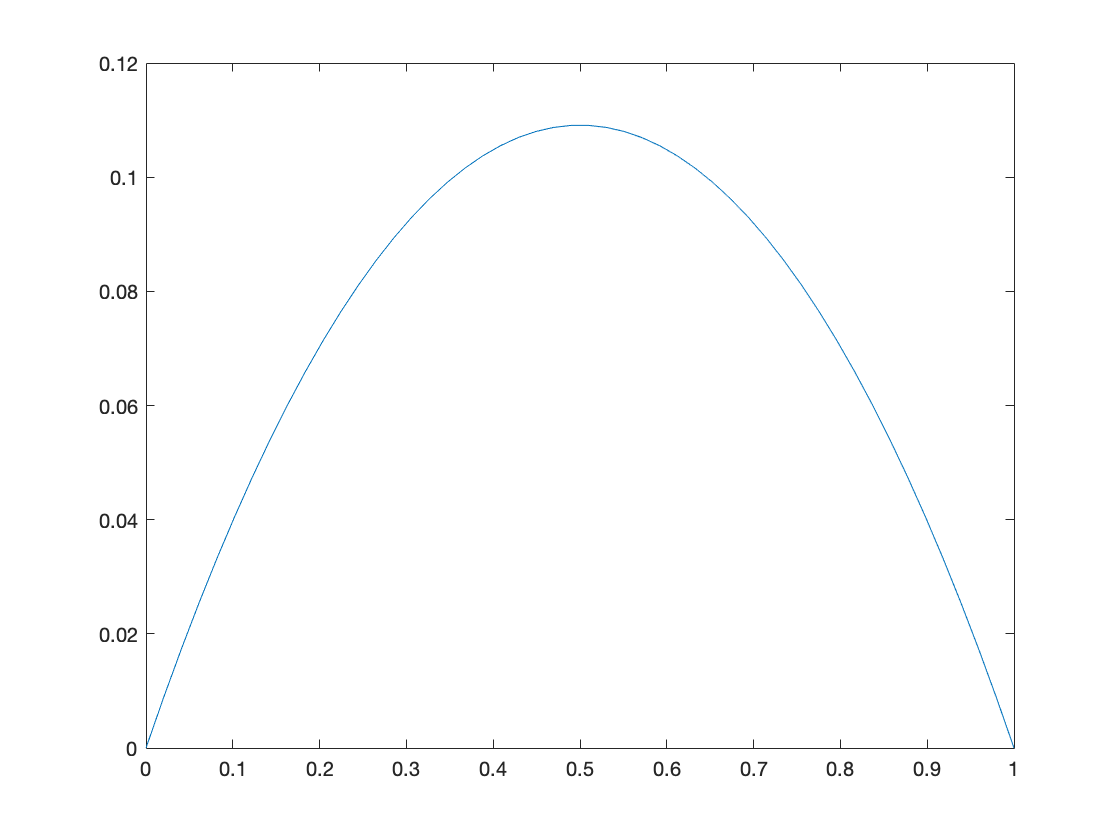
\includegraphics[scale=0.2]{grafica.png}
\end{center}
\end{frame}

\begin{frame}
Consideremos el problema
\begin{align*}
- u^{\prime \prime}(x) + \,u(x) & = 3-2x \text{ para } x \in ]0,1[\\ 
& u(0) = 0  \text{ and } u(1) = 0.  
\end{align*}
Podemos comprobar que la $u(x)=x-x^2$ es una solución de la ecuación. En este 
caso $f(x)=2-3x$ y tenemos que calcular
\begin{align*}
\left\langle 3-2x, w_{i} \right\rangle_{L^2([0,L])} & = \int_0^1 (3-2x) w_k(x) dx \\ 
& =  \int_{x_{i-1}}^{x_i} (3-2x) \frac{x-x_{i-1}}{x_i-x_{i-1}} dx \\ & +
\int_{x_{i}}^{x_{i+1}} (3-2x) \frac{x_{i+1}-x}{x_{i+1}-x_i} dx \\ 
& = \frac{1}{h }\left(\int_{x_{i-1}}^{x_i} (3-2x) (x-x_{i-1}) dx \right. \\ + 
& \left. \int_{x_{i}}^{x_{i+1}} (3-2x) (x_{i+1}-x) dx\right)
\end{align*}
\end{frame}

\begin{frame}{Código Matlab}
\lstinputlisting{ejemplo1.m}
\end{frame}

\begin{frame}
\begin{center}
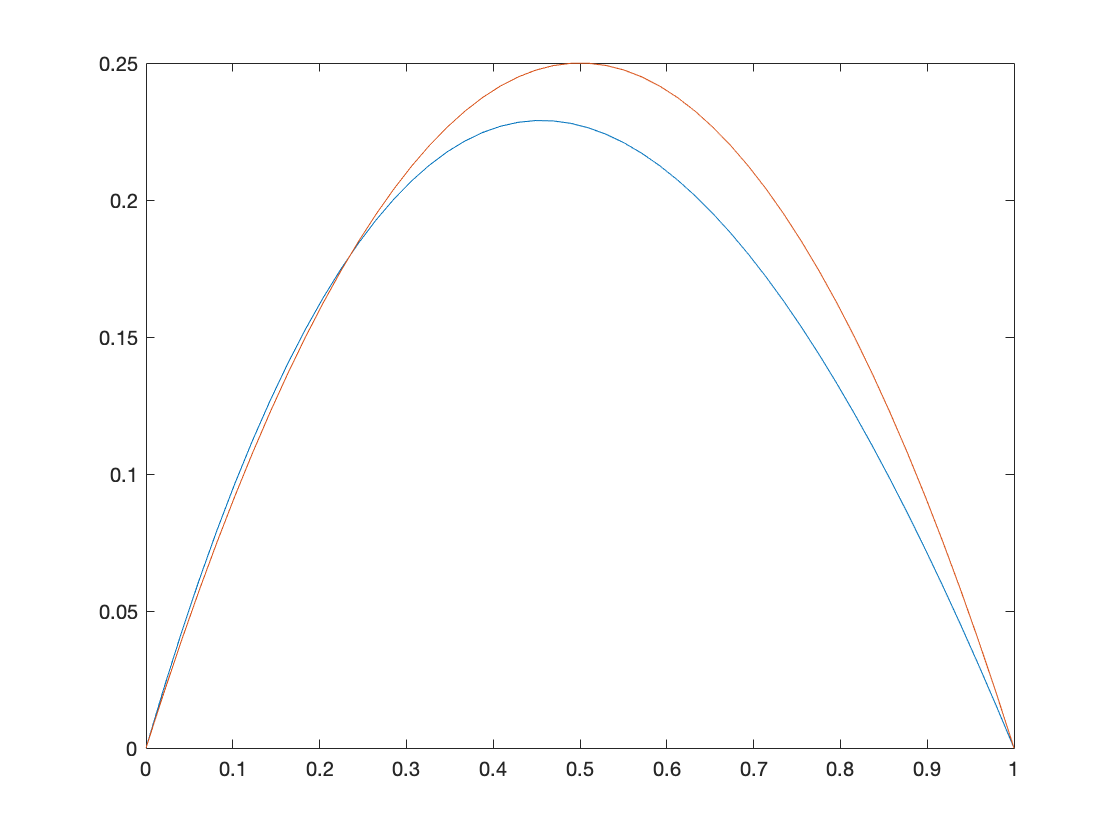
\includegraphics[scale=0.2]{grafica1.png}
\end{center}
\end{frame}

\begin{frame}{Estudio del error de aproximación}
\begin{center}
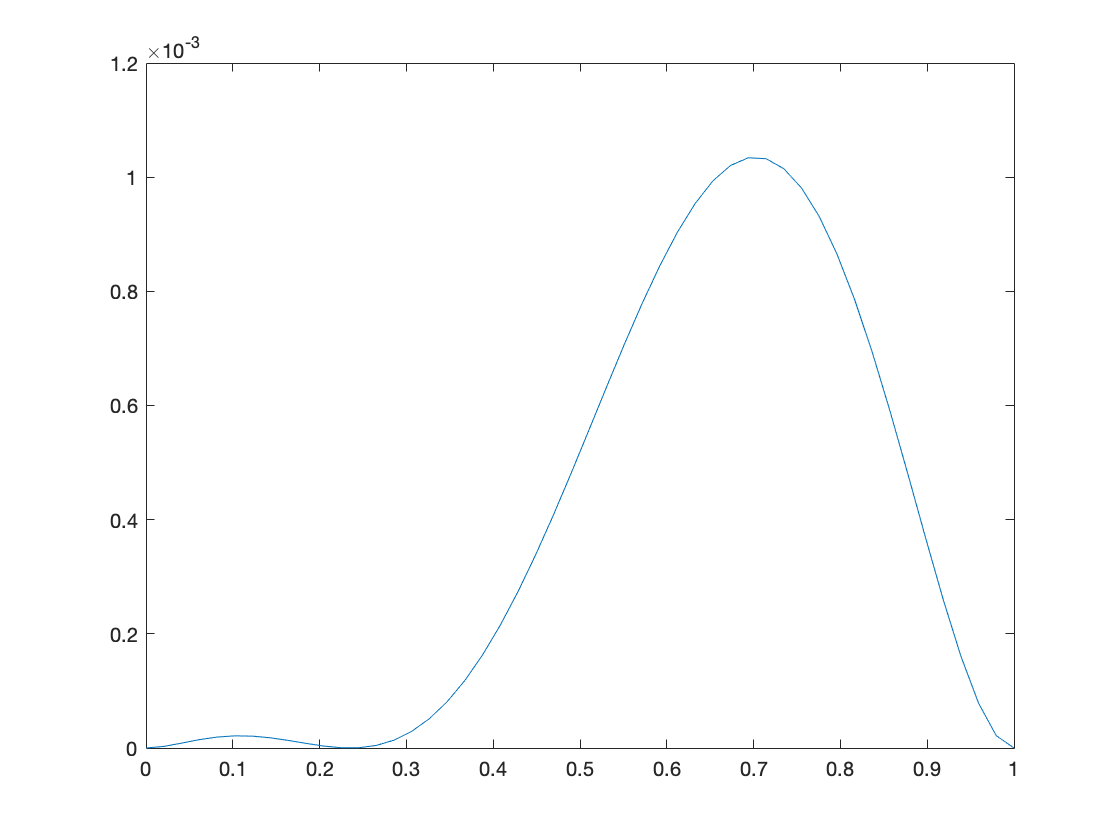
\includegraphics[scale=0.15]{grafica2.png}
\end{center}
Error calculado como $\texttt{error}(i)=(u(x_i)-\widehat{u}_i)^2$. El error
cuadrático medio: $MCE = \frac{1}{d} \sum_{i=1}^d\texttt{error}(i) = 3.8 \times 10^{-4}.$
\end{frame}

\end{document}